% Options for packages loaded elsewhere
\PassOptionsToPackage{unicode}{hyperref}
\PassOptionsToPackage{hyphens}{url}
%
\documentclass[
]{article}
\author{}
\date{\vspace{-2.5em}}

\usepackage{amsmath,amssymb}
\usepackage{lmodern}
\usepackage{iftex}
\ifPDFTeX
  \usepackage[T1]{fontenc}
  \usepackage[utf8]{inputenc}
  \usepackage{textcomp} % provide euro and other symbols
\else % if luatex or xetex
  \usepackage{unicode-math}
  \defaultfontfeatures{Scale=MatchLowercase}
  \defaultfontfeatures[\rmfamily]{Ligatures=TeX,Scale=1}
\fi
% Use upquote if available, for straight quotes in verbatim environments
\IfFileExists{upquote.sty}{\usepackage{upquote}}{}
\IfFileExists{microtype.sty}{% use microtype if available
  \usepackage[]{microtype}
  \UseMicrotypeSet[protrusion]{basicmath} % disable protrusion for tt fonts
}{}
\makeatletter
\@ifundefined{KOMAClassName}{% if non-KOMA class
  \IfFileExists{parskip.sty}{%
    \usepackage{parskip}
  }{% else
    \setlength{\parindent}{0pt}
    \setlength{\parskip}{6pt plus 2pt minus 1pt}}
}{% if KOMA class
  \KOMAoptions{parskip=half}}
\makeatother
\usepackage{xcolor}
\IfFileExists{xurl.sty}{\usepackage{xurl}}{} % add URL line breaks if available
\IfFileExists{bookmark.sty}{\usepackage{bookmark}}{\usepackage{hyperref}}
\hypersetup{
  hidelinks,
  pdfcreator={LaTeX via pandoc}}
\urlstyle{same} % disable monospaced font for URLs
\usepackage[margin=1in]{geometry}
\usepackage{color}
\usepackage{fancyvrb}
\newcommand{\VerbBar}{|}
\newcommand{\VERB}{\Verb[commandchars=\\\{\}]}
\DefineVerbatimEnvironment{Highlighting}{Verbatim}{commandchars=\\\{\}}
% Add ',fontsize=\small' for more characters per line
\usepackage{framed}
\definecolor{shadecolor}{RGB}{248,248,248}
\newenvironment{Shaded}{\begin{snugshade}}{\end{snugshade}}
\newcommand{\AlertTok}[1]{\textcolor[rgb]{0.94,0.16,0.16}{#1}}
\newcommand{\AnnotationTok}[1]{\textcolor[rgb]{0.56,0.35,0.01}{\textbf{\textit{#1}}}}
\newcommand{\AttributeTok}[1]{\textcolor[rgb]{0.77,0.63,0.00}{#1}}
\newcommand{\BaseNTok}[1]{\textcolor[rgb]{0.00,0.00,0.81}{#1}}
\newcommand{\BuiltInTok}[1]{#1}
\newcommand{\CharTok}[1]{\textcolor[rgb]{0.31,0.60,0.02}{#1}}
\newcommand{\CommentTok}[1]{\textcolor[rgb]{0.56,0.35,0.01}{\textit{#1}}}
\newcommand{\CommentVarTok}[1]{\textcolor[rgb]{0.56,0.35,0.01}{\textbf{\textit{#1}}}}
\newcommand{\ConstantTok}[1]{\textcolor[rgb]{0.00,0.00,0.00}{#1}}
\newcommand{\ControlFlowTok}[1]{\textcolor[rgb]{0.13,0.29,0.53}{\textbf{#1}}}
\newcommand{\DataTypeTok}[1]{\textcolor[rgb]{0.13,0.29,0.53}{#1}}
\newcommand{\DecValTok}[1]{\textcolor[rgb]{0.00,0.00,0.81}{#1}}
\newcommand{\DocumentationTok}[1]{\textcolor[rgb]{0.56,0.35,0.01}{\textbf{\textit{#1}}}}
\newcommand{\ErrorTok}[1]{\textcolor[rgb]{0.64,0.00,0.00}{\textbf{#1}}}
\newcommand{\ExtensionTok}[1]{#1}
\newcommand{\FloatTok}[1]{\textcolor[rgb]{0.00,0.00,0.81}{#1}}
\newcommand{\FunctionTok}[1]{\textcolor[rgb]{0.00,0.00,0.00}{#1}}
\newcommand{\ImportTok}[1]{#1}
\newcommand{\InformationTok}[1]{\textcolor[rgb]{0.56,0.35,0.01}{\textbf{\textit{#1}}}}
\newcommand{\KeywordTok}[1]{\textcolor[rgb]{0.13,0.29,0.53}{\textbf{#1}}}
\newcommand{\NormalTok}[1]{#1}
\newcommand{\OperatorTok}[1]{\textcolor[rgb]{0.81,0.36,0.00}{\textbf{#1}}}
\newcommand{\OtherTok}[1]{\textcolor[rgb]{0.56,0.35,0.01}{#1}}
\newcommand{\PreprocessorTok}[1]{\textcolor[rgb]{0.56,0.35,0.01}{\textit{#1}}}
\newcommand{\RegionMarkerTok}[1]{#1}
\newcommand{\SpecialCharTok}[1]{\textcolor[rgb]{0.00,0.00,0.00}{#1}}
\newcommand{\SpecialStringTok}[1]{\textcolor[rgb]{0.31,0.60,0.02}{#1}}
\newcommand{\StringTok}[1]{\textcolor[rgb]{0.31,0.60,0.02}{#1}}
\newcommand{\VariableTok}[1]{\textcolor[rgb]{0.00,0.00,0.00}{#1}}
\newcommand{\VerbatimStringTok}[1]{\textcolor[rgb]{0.31,0.60,0.02}{#1}}
\newcommand{\WarningTok}[1]{\textcolor[rgb]{0.56,0.35,0.01}{\textbf{\textit{#1}}}}
\usepackage{graphicx}
\makeatletter
\def\maxwidth{\ifdim\Gin@nat@width>\linewidth\linewidth\else\Gin@nat@width\fi}
\def\maxheight{\ifdim\Gin@nat@height>\textheight\textheight\else\Gin@nat@height\fi}
\makeatother
% Scale images if necessary, so that they will not overflow the page
% margins by default, and it is still possible to overwrite the defaults
% using explicit options in \includegraphics[width, height, ...]{}
\setkeys{Gin}{width=\maxwidth,height=\maxheight,keepaspectratio}
% Set default figure placement to htbp
\makeatletter
\def\fps@figure{htbp}
\makeatother
\setlength{\emergencystretch}{3em} % prevent overfull lines
\providecommand{\tightlist}{%
  \setlength{\itemsep}{0pt}\setlength{\parskip}{0pt}}
\setcounter{secnumdepth}{-\maxdimen} % remove section numbering
\usepackage{enumitem}
\usepackage{caption}
\usepackage{amsmath}
\captionsetup{labelformat=empty}
\usepackage[utf8]{inputenc}
\usepackage{geometry}
\usepackage{amsmath}
\usepackage{amssymb}
\usepackage{tabularx}
\ifLuaTeX
  \usepackage{selnolig}  % disable illegal ligatures
\fi

\begin{document}

\begin{center}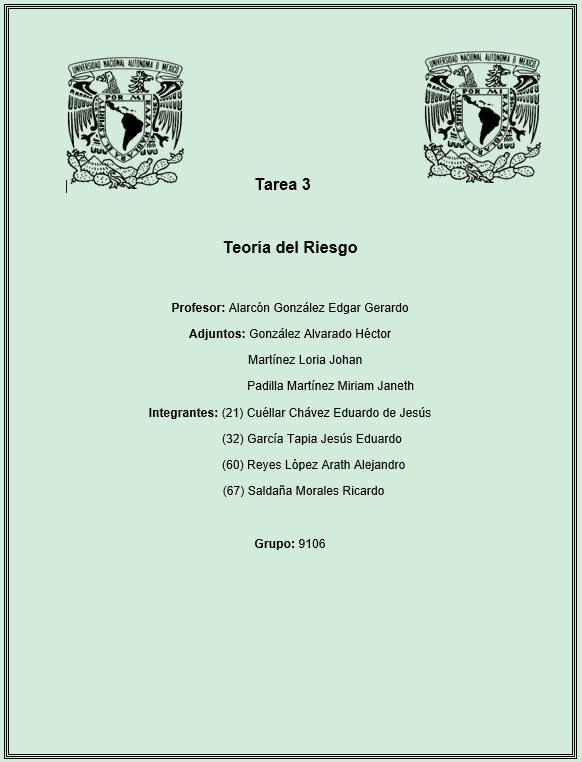
\includegraphics[width=2.4\linewidth]{CARATULA} \end{center}
\newpage

Realiza los siguientes ejercicios cuidando el formato y las reglas
establecidas en la presentación del curso. Sube las soluciones a
\emph{Classroom} dentro del apartado correspondiente a esta tarea en
archivos \textbf{NO COMRPIMIDOS}.

Realiza los siguientes ejercicios entregando el desarrollo algebraico
por escrito (a mano) y las conclusiones del mismo en un archivo de
\textbf{R Markdown con su respectivo compilado PDF} impreso y por correo
electrónico (todos los ejercicios valen lo mismo).

\hypertarget{ejercicio-1}{%
\section{Ejercicio 1}\label{ejercicio-1}}

Sea S un modelo colectivo (compuesto) con frecuencia \(N\sim Bin(n,p)\)
y severidad \(Y\sim Ber(\theta)\). Calcula:

\begin{enumerate}[label=(\alph*)]
\item  $\mathbb{E}[S]$
\item  $Var(S)$
\item  $M_S(t)$
\item Di qué distribución tiene $S$ especificando sus parámetros.
\end{enumerate}

\hypertarget{soluciuxf3n}{%
\subsubsection{Solución}\label{soluciuxf3n}}

\hypertarget{inciso-a}{%
\subsection{Inciso a)}\label{inciso-a}}

Como \begin{align*}
\mathbb{E}[S] &= \mathbb{E}[N] \mathbb{E}[Y]\\
              &= np(\theta)\\
              &= np\theta\\
\therefore \mathbb{E}[S] &= np\theta_\blacksquare
\end{align*}

\hypertarget{inciso-b}{%
\subsection{Inciso b)}\label{inciso-b}}

Como \begin{align*}
Var(S) &= Var(N) \mathbb{E}^{2}(Y) + Var(Y) \mathbb{E}(N)\\
       &= [np(1-p)]\theta^{2} + [\theta(1 - \theta)] np\\
\therefore Var(S) &= [np(1-p)]\theta^{2} + [\theta(1 - \theta)] np_\blacksquare
\end{align*}

\hypertarget{inciso-c}{%
\subsection{Inciso c)}\label{inciso-c}}

Como \begin{align*}
M_{S}(t) &= M_{N} (ln(M_{Y}(t)))\\
\text{Y como} \quad M_{N}(t) &= (1-p + pe^{t})^{n}\\
              M_{Y}(t) &= (1 - \theta + \theta e^{t})\\
              &\implies ln(M_{Y}(t)) = ln(1 - \theta + \theta e^{t})\\
              &\implies M_{S}(t) = (1 - p + p e^{ln(1 - \theta + \theta e^{t})})^{n}\\
              &= (1 - p + p (1 - \theta + \theta e^{t}))^{n}\\
              &= (1 \textcolor{red}{- p + p} - \theta p + \theta p e^{t})^{n}\\
              &= (1 - \theta p + \theta p e^{t})^{n}\\
\therefore M_{S}(t) &= (1 - \theta p + \theta p e^{t})^{n}_\blacksquare
\end{align*}

\hypertarget{inciso-d}{%
\subsection{Inciso d)}\label{inciso-d}}

Notemos que
\(S \sim \text{Binomial compuesta} (n,p,b = Bernoulli(\theta))\)

Además, de manera más especifica;
\(S \sim \text{Binomial}(n, \theta p) \quad \text{por su fmg.}_\blacksquare\)

\hypertarget{ejercicio-2}{%
\section{Ejercicio 2}\label{ejercicio-2}}

Sea S un modelo colectivo (compuesto) con frecuencia
\(N\sim BinNeg(r,p)\) y severidad \(Y\sim Ber(\theta)\). Calcula:

\begin{enumerate}[label=(\alph*)]
\item  $\mathbb{E}[S]$
\item  $Var(S)$
\item  $M_S(t)$
\item Di qué distribución tiene $S$ especificando sus parámetros.
\end{enumerate}

\hypertarget{soluciuxf3n-1}{%
\subsubsection{Solución}\label{soluciuxf3n-1}}

\hypertarget{inciso-a-1}{%
\subsection{Inciso a)}\label{inciso-a-1}}

Como \begin{align*}
\mathbb{E}[S] &= \mathbb{E}[N] \mathbb{E}[Y]\\
              &= \frac{r (1 - p)}{p}(\theta)\\
              &= r\theta \left(\frac{1}{p} - 1\right)\\
\therefore \mathbb{E}[S] &= r\theta \left(\frac{1}{p} - 1\right)_\blacksquare
\end{align*}

\hypertarget{inciso-b-1}{%
\subsection{Inciso b)}\label{inciso-b-1}}

Como \begin{align*}
Var(S) &= Var(N) \mathbb{E}^{2}(Y) + Var(Y) \mathbb{E}(N)\\
       &= \frac{r(1 - p)}{p^{2}}\theta^{2} + [\theta(1 - \theta)] \frac{r (1 - p)}{p}\\
\therefore Var(S) &= \frac{r(1 - p)}{p^{2}}\theta^{2} + [\theta(1 - \theta)] \frac{r (1 - p)}{p}_\blacksquare
\end{align*}

\hypertarget{inciso-c-1}{%
\subsection{Inciso c)}\label{inciso-c-1}}

Como \begin{align*}
M_{S}(t) &= M_{N} (ln(M_{Y}(t)))\\
\text{Y como} \quad M_{N}(t) &= \left[\frac{p}{1 - (1 - p)e^{t}}\right]^{r}\\
              M_{Y}(t) &= (1 - \theta + \theta e^{t})\\
              &\implies ln(M_{Y}(t)) = ln(1 - \theta + \theta e^{t})\\
              &\implies M_{S}(t) = \left[\frac{p}{1 - (1 - p) e^{ln(1 - \theta + \theta e^{t})}}\right]^{r}
\end{align*} \begin{align*}
              &= \left[\frac{p}{1 - (1 - p) \left[1 - \theta + \theta e^{t}\right]}\right]^{r}\\
\therefore M_{S}(t) &= \left[\frac{p}{1 - (1 - p) \left[1 - \theta + \theta e^{t}\right]}\right]^{r}_\blacksquare\\
\text{Notemos los siguiente:}\\
M_{S}(t) &= \left[\frac{p}{1 - (1 - p) \left[1 - \theta + \theta e^{t}\right]}\right]^{r}\\
&= \left[\frac{p}{1 - (1 - p)(1 - \theta) - (1 - p)\theta e^{t}}\right]^{r}\\
&= \left[\frac{\frac{p}{1 - (1 - p)(1 - \theta)}}{\frac{1 - (1 - p)(1 - \theta) - (1 - p)\theta e^{t}}{1 - (1 - p)(1 - \theta)}}\right]^{r}\\
&= \left[\frac{\frac{p}{1 - (1 - p)(1 - \theta)}}{1 - \frac{(1 - p)\theta e^{t}}{1 - (1 - p)(1 - \theta)}}\right]^{r}\\
&= \left[\frac{\frac{p}{1 - (1 - p)(1 - \theta)}}{1 - \left[1 - \frac{p}{1 - (1 - p)(1 - \theta)}\right]e^{t}}\right]^{r}\\
\left[\alpha = \frac{p}{1 - (1 - p)(1 - \theta)}\right] &= \left(\frac{\alpha}{1 - (1 - \alpha)e^{t}}\right)^{r}\\
&\therefore S \sim \text{Binomial Negativa}(r, \alpha)_\blacksquare
\end{align*}

\hypertarget{inciso-d-1}{%
\subsection{Inciso d)}\label{inciso-d-1}}

\textcolor{red}{Como ya vimos en c), encontramos la distribución de $S$, para confirmar veamos que sucede con la densidad de $S$ en términos de $N$ y $Y$.}

Sea
\(N \sim \text{Binomial Negativa} (r,p) \quad \text{y}\quad Y \sim Bernoulli(\theta)\),
es decir;

\begin{align*}
S &= \sum_{i = 1}^{N}Y_{i}; S|N = n \sim Bin(n,\theta)\\
\implies \mathbb{P}(S = k) &= \sum_{n = k}^{\infty} \mathbb{P}(S = K | N = n)\mathbb{P}(N = n)\\
\text{Sea} \quad Q = (1 - P) &= \sum_{n=k}^{\infty} \binom{n}{k} \theta^{k} (1 -  \theta)^{n-k} \binom{n + r - 1}{n}(1 - Q)^{r}Q^{n}\\
&= (1 - Q)^{r} \sum_{n = k}^{\infty} \left(\frac{\textcolor{red}{n!}}{k! (n - k)!}\right)\left(\frac{(n + r - 1)!}{\textcolor{red}{n!}(r-1)!}\right) Q^{n}\textcolor{red}{\theta^{k}} \frac{(1 - \theta)^{n}}{(1 - \theta)^{k}}\\
&= \frac{(1 - Q)^{r}}{k! (r - 1)!} \left(\frac{\theta}{1 - \theta}\right)^{k} \sum_{n = k}^{\infty} \frac{(n + r - 1)!}{(n - k)!}(Q(1 - \theta))^{n}\\
\text{Haciendo cambio de variable,} u = n-k\\
&= \frac{(1 - Q)^{r}}{(k!)(r - 1)!}\left(\frac{\theta}{1 - \theta}\right)^{k} \sum_{u = 0}^{\infty} \frac{(u + k + r - 1)!}{u!}(Q(1 - \theta))^{u+k}\\
&= \frac{(1 - Q)^{r}}{k!(r - 1)!}(Q \theta)^{k} \sum_{u = 0}^{\infty} \underbrace{\frac{(u + k + r - 1)!}{u!}(Q(1 - \theta))^{u}}_{1}
\end{align*} \begin{align*}
x = Q(1 - \theta); x \in (0,1)\\
&\implies \sum_{u = 0}^{\infty} x^{u} = \frac{1}{1 - x}  \quad \underrightarrow{dx} \quad \sum_{u = 0}^{\infty} ux^{u - 1}  = \frac{1}{(1 - x)^{2}}\\
= \sum_{u = 0}^{\infty} u x^{u - 1} &= \frac{1}{(1 - x)^{2}} \quad \underrightarrow{dx} \quad \sum_{u = 1}^{\infty} u(u - 1) x^{u - 2} = \sum_{u = 2}^{\infty} u(u - 1) x^{u - 2}\\
&= \frac{2}{(1 - x)^{3}}, \quad \text{Continuando inductivamente se llega a que:}\\
&\implies \sum_{u = K + r - 1}^{\infty} \left[\frac{u!}{(u - (k + r - 1))!}\right] X^{u + 1 - k - r} = \frac{(k + r - 1)!}{(1 - x)^{k + r}}\\
i = u - (k + r - 1)\\
&\implies \underbrace{\sum_{i = 0}^{\infty} \frac{(i + k + r -1)!}{i!} x^{i}}_{1} = \frac{(k + r - 1)!}{(1 - X)^{k + r}}\\
&\implies \sum_{u = 0}^{\infty} \frac{(u + k + r - 1)!}{u!} (Q(1 - \theta))^{u} = \frac{(k + r - 1)!}{(1 - Q(1 - \theta))^{k+ r}}\\
\implies \mathbb{P}(S = k) &= \frac{(1 - Q)^{r}}{K! (r - 1)!}(Q\theta)^{k} \frac{(K + r -1)!}{(1 - Q (1 - \theta))^{k + r}}\\
&= \binom{k + r - 1}{k} \left(\frac{Q\theta}{1 - Q(1 - \theta)}\right)^{k} \left(\frac{1 - Q}{1 - Q(1 - \theta)}\right)^{r}\\
\left(\alpha = \frac{1 - Q}{1 - Q(1 - \theta)} = \frac{P}{1 - (1 - P)(1 - \theta)}\right) &= \binom{k + r -1}{k} (1 - \alpha)^{k} \alpha^{r} \quad \forall k \in \mathbb{N}\cup\{0\}\\
&\therefore S \sim \text{Binomial Negativa}(r, \alpha)_\blacksquare
\end{align*}

\textbf{\textcolor{red}{NOTA:}} Es necesario que todas las series
convergan uniformemente para meter la diferencial dentro de la serie, lo
cual es cierto por el teorema 5.28 del Clapp que nos asegura toda serie
de potencias converge uniformemente y en consecuencia es diferenciable.

\hypertarget{ejercicio-3}{%
\section{Ejercicio 3}\label{ejercicio-3}}

Considera los siguientes 3 riesgos de una compañía:

\[S_j\sim\text{PoiComp}\left(\lambda_j=j^2,F_{Y_j}\right)\]

Donde las severidades están dadas por:

\begin{itemize}
\tightlist
\item
  \(F_{Y_1}(y)=1-e^{-0.5y} \mathbb{I}^{(y)}_{\{y>0\}}\)
\item
  \(Y_2\) pertenece a la clase (a,b,0) con: \(a=0.1\) , \(b=2(0.1)\) y
  \(p_0=(0.9)^{3}\)
\item
  \(Y_3\) es la v.a. del monto de pérdida de una compañía de seguros con
  un \textbf{contrato de monto máximo de beneficio} \(u=50\) donde el
  monto de pérdida del siniestro es
  \(X\sim Exp\left(\lambda=\frac{1}{100}\right)\) (\(E[X]=100\)).
\end{itemize}

Define el riesgo \(S\) de la compañía como:

\[S=\sum_{j=1}^{3} S_j\]

\textbf{Fija la semilla en 6}, simula \(n=1,000,000\) observaciones de
\(S\) y calcula de manera muestral:

\begin{enumerate}[label=(\alph*)]
\item  El coeficiente de variación de $S$.
\item  Un valor $z$ tal que $F_S(500)\approx \Phi(z)$.
\end{enumerate}

\hypertarget{soluciuxf3n-2}{%
\subsubsection{Solución}\label{soluciuxf3n-2}}

\textcolor{red}{Observaciones:}

\begin{align*}
a &= 0.1 \epsilon (0,1)\\
b &= 2(0.1) \geq 0\\
p_{0} &= (0.9)^{3}\\
&\therefore \text{Es Binomial Negativa con p = 0.9 y r = 3}
\end{align*}

Por otro lado, \begin{align*}
F_{Y}(Y) &= 1 - e^{-0.5_{Y}} \mathbb{I}_{\{Y > 0\}}^{(y)}\\
&\therefore \text{Es Exponencial} \quad \lambda = 0.5 = \frac{1}{2}
\end{align*}

Finalmente veamos que; \(Y_{3} = mín(exp(\frac{1}{100})50)\)

Por otro lado, haciendo uso de Dart Vader;

\begin{align*}
& \int_{0}^{50} S(x)dx\\
&= \int_{0}^{50} e^{-\lambda x} + 50e^{-\lambda(50)} = -\frac{e^{-\lambda x}}{\lambda}|_{0}^{50}\\
&= - \left(\frac{e^{-\lambda(50)}}{\lambda} - \frac{1}{\lambda}\right) + 50 * e^{-\lambda(50)}\\
&= \frac{1}{\lambda} + e^{-\lambda(50)}(50 - \frac{1}{\lambda})
\end{align*}

\textcolor{red}{Así, a continuación el código, que da respuesta a los incisos a y b}

\begin{Shaded}
\begin{Highlighting}[]
\FunctionTok{library}\NormalTok{(actuar)}
\NormalTok{n }\OtherTok{\textless{}{-}} \DecValTok{1000000}
\FunctionTok{set.seed}\NormalTok{(}\DecValTok{6}\NormalTok{)}

\CommentTok{\#Parámetro de la Poisson}
\NormalTok{lambda1 }\OtherTok{\textless{}{-}} \DecValTok{1}\SpecialCharTok{\^{}}\DecValTok{2}
\NormalTok{lambda2 }\OtherTok{\textless{}{-}} \DecValTok{2}\SpecialCharTok{\^{}}\DecValTok{2}
\NormalTok{lambda3 }\OtherTok{\textless{}{-}} \DecValTok{3}\SpecialCharTok{\^{}}\DecValTok{2}
\NormalTok{lambda }\OtherTok{\textless{}{-}}\NormalTok{ lambda1 }\SpecialCharTok{+}\NormalTok{ lambda2 }\SpecialCharTok{+}\NormalTok{ lambda3}

\CommentTok{\#Exponencial}
\NormalTok{rate\_1 }\OtherTok{\textless{}{-}} \DecValTok{1}\SpecialCharTok{/}\DecValTok{2}
\NormalTok{S1 }\OtherTok{\textless{}{-}} \FunctionTok{rcompound}\NormalTok{(}\AttributeTok{n =}\NormalTok{ n, }\CommentTok{\#Genera n}
               \AttributeTok{model.freq =} \FunctionTok{rpois}\NormalTok{(}\AttributeTok{lambda =}\NormalTok{ lambda1), }\CommentTok{\#N\textasciitilde{}Poi(lambda2)}
               \AttributeTok{model.sev =} \FunctionTok{rexp}\NormalTok{(}\AttributeTok{rate =}\NormalTok{ rate\_1)) }\CommentTok{\#Y\textasciitilde{}Exp(rate) }

\CommentTok{\#Binomial negativa}
\NormalTok{r}\OtherTok{=}\DecValTok{3}
\NormalTok{p}\OtherTok{=}\FloatTok{0.9}
\NormalTok{S2 }\OtherTok{\textless{}{-}} \FunctionTok{rcompound}\NormalTok{(}\AttributeTok{n =}\NormalTok{ n, }\CommentTok{\#Genera n}
                \AttributeTok{model.freq =} \FunctionTok{rpois}\NormalTok{(}\AttributeTok{lambda =}\NormalTok{ lambda2), }\CommentTok{\#N\textasciitilde{}Poi(lambda1)}
                \AttributeTok{model.sev =} \FunctionTok{rnbinom}\NormalTok{(}\AttributeTok{size =}\NormalTok{ r,}\AttributeTok{p=}\NormalTok{p)) }\CommentTok{\#Y\textasciitilde{}NegBinom(r=3,p=0.9) }

\CommentTok{\#Exponencial topada}
\NormalTok{rate\_2}\OtherTok{\textless{}{-}} \DecValTok{1}\SpecialCharTok{/}\DecValTok{100}
\NormalTok{u}\OtherTok{=}\DecValTok{50}
\NormalTok{aux}\OtherTok{\textless{}{-}}\ControlFlowTok{function}\NormalTok{(n,rate,u)\{ }\CommentTok{\#Exponencial topada a 50}
  \FunctionTok{return}\NormalTok{(}\FunctionTok{pmin}\NormalTok{(}\FunctionTok{rexp}\NormalTok{(}\AttributeTok{n=}\NormalTok{n,}\AttributeTok{rate=}\NormalTok{rate),u))}
\NormalTok{\}}
\NormalTok{S3 }\OtherTok{\textless{}{-}} \FunctionTok{rcompound}\NormalTok{(}\AttributeTok{n =}\NormalTok{ n, }\CommentTok{\#Genera n}
                \AttributeTok{model.freq =} \FunctionTok{rpois}\NormalTok{(}\AttributeTok{lambda =}\NormalTok{ lambda3), }\CommentTok{\#N\textasciitilde{}Poi(lambda3)}
                \AttributeTok{model.sev =} \FunctionTok{aux}\NormalTok{(}\AttributeTok{rate=}\NormalTok{rate\_2,u)) }\CommentTok{\#Y:=min(Exp(1/100),50)}
\NormalTok{S }\OtherTok{\textless{}{-}}\NormalTok{ S1 }\SpecialCharTok{+}\NormalTok{ S2 }\SpecialCharTok{+}\NormalTok{ S3}

\CommentTok{\#Teórica}
\NormalTok{mu\_nbinom}\OtherTok{=}\NormalTok{r}\SpecialCharTok{*}\NormalTok{(}\DecValTok{1}\SpecialCharTok{/}\NormalTok{p}\DecValTok{{-}1}\NormalTok{)}
\NormalTok{mu\_exp}\OtherTok{=}\DecValTok{1}\SpecialCharTok{/}\NormalTok{rate\_1}
\NormalTok{mu\_exp\_topada}\OtherTok{=}\DecValTok{1}\SpecialCharTok{/}\NormalTok{rate\_2}\SpecialCharTok{{-}}\FunctionTok{exp}\NormalTok{(}\SpecialCharTok{{-}}\NormalTok{rate\_2}\SpecialCharTok{*}\NormalTok{u)}\SpecialCharTok{/}\NormalTok{rate\_2;mu\_exp\_topada}
\end{Highlighting}
\end{Shaded}

\begin{verbatim}
## [1] 39.34693
\end{verbatim}

\begin{Shaded}
\begin{Highlighting}[]
\FunctionTok{mean}\NormalTok{(}\FunctionTok{aux}\NormalTok{(}\DecValTok{5000}\NormalTok{,}\AttributeTok{rate=}\NormalTok{rate\_2,u))}
\end{Highlighting}
\end{Shaded}

\begin{verbatim}
## [1] 39.32978
\end{verbatim}

\begin{Shaded}
\begin{Highlighting}[]
\NormalTok{mu}\OtherTok{\textless{}{-}}\NormalTok{lambda}\SpecialCharTok{*}\NormalTok{(lambda1}\SpecialCharTok{*}\NormalTok{mu\_nbinom }\SpecialCharTok{+}  \CommentTok{\#Esperanza de la binomial negativa}
\NormalTok{        lambda2}\SpecialCharTok{*}\NormalTok{mu\_exp }\SpecialCharTok{+} \CommentTok{\#Esperanza de la exponencial}
\NormalTok{        lambda3}\SpecialCharTok{*}\NormalTok{mu\_exp\_topada }\CommentTok{\#Esperanza de la exponencial topada}
\NormalTok{        )}\SpecialCharTok{/}\NormalTok{lambda ; mu}
\end{Highlighting}
\end{Shaded}

\begin{verbatim}
## [1] 362.4557
\end{verbatim}

\begin{Shaded}
\begin{Highlighting}[]
\CommentTok{\#Muestral}
\NormalTok{mu\_muestral}\OtherTok{\textless{}{-}}\FunctionTok{mean}\NormalTok{(S)}

\CommentTok{\#Coinciden!}

\CommentTok{\#Teorica }

\CommentTok{\#2do momento de la binomial negativa}
\NormalTok{mu\_2\_nbinom}\OtherTok{=}\NormalTok{(r}\SpecialCharTok{*}\NormalTok{(}\DecValTok{1}\SpecialCharTok{{-}}\NormalTok{p)}\SpecialCharTok{/}\NormalTok{p}\SpecialCharTok{\^{}}\DecValTok{2}\SpecialCharTok{+}\NormalTok{(r}\SpecialCharTok{*}\NormalTok{(}\DecValTok{1}\SpecialCharTok{{-}}\NormalTok{p)}\SpecialCharTok{/}\NormalTok{p)}\SpecialCharTok{\^{}}\DecValTok{2}\NormalTok{)}
\CommentTok{\#2do momento de la Exponencial}
\NormalTok{mu\_2\_exp}\OtherTok{=}\NormalTok{(}\DecValTok{2}\SpecialCharTok{/}\NormalTok{rate\_1}\SpecialCharTok{\^{}}\DecValTok{2}\NormalTok{)}
\CommentTok{\#2do momento de la Exponencial topada}
\NormalTok{mu\_2\_exp\_topada}\OtherTok{=}\NormalTok{((}\FunctionTok{exp}\NormalTok{(}\SpecialCharTok{{-}}\NormalTok{rate\_2}\SpecialCharTok{*}\NormalTok{u)}\SpecialCharTok{*}\NormalTok{(}\SpecialCharTok{{-}}\NormalTok{rate\_2}\SpecialCharTok{*}\NormalTok{u}\SpecialCharTok{*}\NormalTok{(rate\_2}\SpecialCharTok{*}\NormalTok{u}\SpecialCharTok{+}\DecValTok{2}\NormalTok{)}\SpecialCharTok{{-}}\DecValTok{2}\NormalTok{)}\SpecialCharTok{+}\DecValTok{2}\NormalTok{)}\SpecialCharTok{/}\NormalTok{rate\_2}\SpecialCharTok{\^{}}\DecValTok{2}\SpecialCharTok{+}\NormalTok{(}\DecValTok{50}\SpecialCharTok{\^{}}\DecValTok{2}\NormalTok{)}\SpecialCharTok{*}\FunctionTok{exp}\NormalTok{(}\SpecialCharTok{{-}}\NormalTok{rate\_2}\SpecialCharTok{*}\DecValTok{50}\NormalTok{))}
\NormalTok{var}\OtherTok{\textless{}{-}}\NormalTok{lambda}\SpecialCharTok{*}\NormalTok{(}
\NormalTok{        lambda1}\SpecialCharTok{*}\NormalTok{mu\_2\_nbinom }\SpecialCharTok{+} 
\NormalTok{        lambda2}\SpecialCharTok{*}\NormalTok{mu\_2\_exp }\SpecialCharTok{+}
\NormalTok{        lambda3}\SpecialCharTok{*}\NormalTok{mu\_2\_exp\_topada}
\NormalTok{        )}\SpecialCharTok{/}\NormalTok{lambda;var}
\end{Highlighting}
\end{Shaded}

\begin{verbatim}
## [1] 16269.2
\end{verbatim}

\begin{Shaded}
\begin{Highlighting}[]
\NormalTok{var\_muestral}\OtherTok{\textless{}{-}}\FunctionTok{var}\NormalTok{(S)}
\end{Highlighting}
\end{Shaded}

El coeficiente de variación es:

\begin{Shaded}
\begin{Highlighting}[]
\NormalTok{Coeficiente\_variacion}\OtherTok{\textless{}{-}}\FunctionTok{sd}\NormalTok{(S)}\SpecialCharTok{/}\FunctionTok{abs}\NormalTok{(}\FunctionTok{mean}\NormalTok{(S))}
\NormalTok{Coeficiente\_variacion}
\end{Highlighting}
\end{Shaded}

\begin{verbatim}
## [1] 0.3565534
\end{verbatim}

\(\blacksquare\)

Un valor de z tal que \(F_s(500)\approx \Phi (z)\):

\begin{Shaded}
\begin{Highlighting}[]
\NormalTok{z}\OtherTok{\textless{}{-}}\NormalTok{(}\DecValTok{500}\SpecialCharTok{{-}}\FunctionTok{mean}\NormalTok{(S))}\SpecialCharTok{/}\FunctionTok{sd}\NormalTok{(S)}
\NormalTok{z}
\end{Highlighting}
\end{Shaded}

\begin{verbatim}
## [1] 1.118446
\end{verbatim}

\begin{Shaded}
\begin{Highlighting}[]
\FunctionTok{pnorm}\NormalTok{(z)}
\end{Highlighting}
\end{Shaded}

\begin{verbatim}
## [1] 0.8683117
\end{verbatim}

\begin{Shaded}
\begin{Highlighting}[]
\FunctionTok{quantile}\NormalTok{(S,}\FunctionTok{pnorm}\NormalTok{(z))}
\end{Highlighting}
\end{Shaded}

\begin{verbatim}
## 86.83117% 
##  501.9658
\end{verbatim}

\(\blacksquare\)

\hypertarget{ejercicio-4}{%
\section{Ejercicio 4}\label{ejercicio-4}}

El monto agregado de \(S\) de un riesgo tiene distribución binomial
compuesta \(N\sim Bin(n=10,p=0.4)\) donde los montos de reclamación
tienen una función de masa de probabilidad:

\[ 
f_X(x)=\mathbb{P}[X=x]
\begin{cases}
0.40 \quad, \hspace{0.8cm} \text{si} \hspace{0.4cm} x = 1\\
0.35  \quad, \hspace{0.8cm} \text{si} \hspace{0.4cm} x=2\\
0.25  \quad, \hspace{0.8cm} \text{si} \hspace{0.4cm} x=3
\end{cases}
\]

\begin{enumerate}[label=(\alph*)]
\item Calcula $\mathbb{P}[S\leq 5]$
\item Calcula $\mathbb{P}[S = 6]$
\end{enumerate}

\hypertarget{soluciuxf3n-3}{%
\subsubsection{Solución}\label{soluciuxf3n-3}}

\hypertarget{inciso-a-2}{%
\subsection{Inciso a)}\label{inciso-a-2}}

Notemos que: \(-\frac{0.4}{0.6} = -\frac{2}{3} = a\) y que
\(\frac{11(0.4)}{0.6} = \frac{22}{3} = b\) \begin{align*}
\mathbb{P}(S = 0) &= \mathbb{P}(N = 0) = 0.6^{10}\\
\mathbb{P}(S = 1) &= \left(a + \frac{b(1)}{1}\right)0.4[0.6]^{10} = \left(\frac{22}{3} - \frac{2}{3}\right)0.4[0.6]^{10}\\
&\approx 0.016124314\\
\mathbb{P}(S = 2) &= \left(a + \frac{b(1)}{2}\right)\mathbb{P}(X = 1)\mathbb{P}(S = 2 - 1)\\
&+  \left(a + \frac{b(2)}{2}\right)\mathbb{P}(X = 2)\mathbb{P}(S = 2 - 2)
\end{align*} \begin{align*}
&=(a + \frac{b}{2})0.4[0.016124314]\\
&+ (a + b)0.35[0.6]^{10}\\
&= (\frac{11}{3} - \frac{2}{3})0.4[0.016124314]\\
&+ (\frac{20}{3})0.35[0.6]^{10}\\
&= 0.033457951\\
\mathbb{P}(S = 3) &= \left(a + \frac{b(1)}{3}\right)\mathbb{P}(X = 1)\mathbb{P}(S = 3 - 1)\\
&+  \left(a + \frac{b(2)}{3}\right)\mathbb{P}(X = 2)\mathbb{P}(S = 3 - 2)\\
&+ \left(a + \frac{b(3)}{3}\right)\mathbb{P}(X = 3)\mathbb{P}(S = 3 - 3)\\
&= \left(-\frac{2}{3} + \frac{22}{9}\right)0.4[0.033457951]\\
&+ \left(-\frac{2}{3} + \frac{44}{9}\right)0.35[0.016124314]\\
&+ \left(-\frac{2}{3} + \frac{22}{3}\right)0.25[0.6^{10}]\\
&= 0.05769817\\
\mathbb{P}(S = 4) &= \left(a + \frac{b(1)}{4}\right)\mathbb{P}(X = 1)\mathbb{P}(S = 4 - 1)\\
&+  \left(a + \frac{b(2)}{4}\right)\mathbb{P}(X = 2)\mathbb{P}(S = 4 - 2)\\
&+ \left(a + \frac{b(3)}{4}\right)\mathbb{P}(X = 3)\mathbb{P}(S = 4 - 3)\\
&= \left(-\frac{2}{3} + \frac{22}{12}\right)0.4[0.05769817]\\
&+ \left(-\frac{2}{3} + \frac{11}{3}\right)0.35[0.033457951]\\
&+ \left(-\frac{2}{3} + \frac{11}{2}\right)0.25[0.016124314]\\
&= 0.081540207\\
\mathbb{P}(S = 5) &= \left(a + \frac{b(1)}{5}\right)0.4\mathbb{P}(S = 5 - 1)\\
&+  \left(a + \frac{b(2)}{5}\right)0.35\mathbb{P}(S = 5 - 2)\\
&+ \left(a + \frac{b(3)}{5}\right)0.25\mathbb{P}(S = 5 - 3)\\
&= \left(-\frac{2}{3} + \frac{22}{15}\right)0.4[0.081540207]\\
&+ \left(-\frac{2}{3} + \frac{44}{15}\right)0.35[0.05769817]\\
&+ \left(-\frac{2}{3} + \frac{22}{5}\right)0.25[0.033457951]\\
&= 0.103094169
\end{align*} \begin{align*}
\mathbb{P}(S = 6) &= \left(a + \frac{b(1)}{6}\right)0.4\mathbb{P}(S = 6 - 1)\\
&+ \left(a + \frac{b(2)}{6}\right)0.35\mathbb{P}(S = 6 - 2)\\
&+ \left(a + \frac{b(3)}{6}\right)0.25\mathbb{P}(S = 6 - 3)\\
&= \left(-\frac{2}{3} + \frac{11}{9}\right)0.4[0.103094169]\\
&+ \left(-\frac{2}{3} + \frac{22}{9}\right)0.35[0.081540207]\\
&+ \left(-\frac{2}{3} + \frac{11}{3}\right)0.25[0.05769817]\\
&= 0.116919572
\end{align*}

De esta manera se obtiene que: \begin{align*}
&\textcolor{red}{\mathbb{P}(S = 6) = 0.116919572}\\
&\textcolor{red}{y}\\
&\textcolor{red}{\mathbb{P}(S \leq 5)} = \mathbb{P}(S = 0) + \mathbb{P}(S = 1) + \dots + \mathbb{P}(S = 5)\\
&= 0.6^{10} + 0.016124314 + 0.033457951\\
&+ 0.05769817 0.081540207 + 0.103094169\\
&= 0.297961428\\
&\textcolor{red}{\therefore \mathbb{P}(S \leq 5) = .297961428}_\blacksquare
\end{align*}

Además podemos confirmar nuestros resultados con el siguiente código:

\begin{Shaded}
\begin{Highlighting}[]
\DocumentationTok{\#\#Probabilidades reales}
\NormalTok{Panjer }\OtherTok{\textless{}{-}} \ControlFlowTok{function}\NormalTok{(x,p0,a,b,f)\{}
  
  \CommentTok{\# x := Valor al que se le desea calcular la probabilidad de P[S=x]}
  \CommentTok{\#p0 := Probabilidad en 0 de N}
  \CommentTok{\# (a,b) := Parametros de la familia (a,b,0)}
  \CommentTok{\#f := vector de probabilidades de X}
  
  \CommentTok{\#Creamos un vector auxiliar para las probas de S.}
\NormalTok{  g}\OtherTok{\textless{}{-}}\DecValTok{0}\SpecialCharTok{:}\NormalTok{x}
  \FunctionTok{names}\NormalTok{(g)}\OtherTok{\textless{}{-}}\DecValTok{0}\SpecialCharTok{:}\NormalTok{x}
  
  \CommentTok{\#Le ponemos nombres al vector de probas de f.}
  \FunctionTok{names}\NormalTok{(f)}\OtherTok{\textless{}{-}}\DecValTok{1}\SpecialCharTok{:}\FunctionTok{length}\NormalTok{(f)}
  
  \CommentTok{\#Panjer (de clase (a,b,0) con soporte de Xj sin 0)}
  \ControlFlowTok{for}\NormalTok{(s }\ControlFlowTok{in} \DecValTok{0}\SpecialCharTok{:}\NormalTok{x)\{}
    \ControlFlowTok{if}\NormalTok{(s}\SpecialCharTok{==}\DecValTok{0}\NormalTok{)\{}
\NormalTok{      g[}\StringTok{"0"}\NormalTok{]}\OtherTok{=}\NormalTok{p0}
\NormalTok{    \}}\ControlFlowTok{else}\NormalTok{\{aux }\OtherTok{=} \DecValTok{0}
    \ControlFlowTok{for}\NormalTok{(j }\ControlFlowTok{in} \DecValTok{1}\SpecialCharTok{:}\NormalTok{(}\FunctionTok{min}\NormalTok{(s,}\FunctionTok{length}\NormalTok{(f)}\SpecialCharTok{{-}}\DecValTok{1}\NormalTok{)))\{}
\NormalTok{      aux }\OtherTok{=}\NormalTok{ aux }\SpecialCharTok{+}\NormalTok{ (a }\SpecialCharTok{+}\NormalTok{ ((b}\SpecialCharTok{*}\NormalTok{j)}\SpecialCharTok{/}\NormalTok{s))}\SpecialCharTok{*}\NormalTok{f[}\FunctionTok{as.character}\NormalTok{(j)]}\SpecialCharTok{*}\NormalTok{g[}\FunctionTok{as.character}\NormalTok{(s}\SpecialCharTok{{-}}\NormalTok{j)]}
\NormalTok{    \}}
\NormalTok{    g[}\FunctionTok{as.character}\NormalTok{(s)]}\OtherTok{=}\NormalTok{aux}
\NormalTok{    \}}
\NormalTok{  \}}
  \FunctionTok{names}\NormalTok{(g)}\OtherTok{\textless{}{-}}\FunctionTok{paste}\NormalTok{(}\StringTok{"P[S="}\NormalTok{,}\FunctionTok{names}\NormalTok{(g),}\StringTok{"]"}\NormalTok{,}\AttributeTok{sep =} \StringTok{""}\NormalTok{)}
  
  \FunctionTok{return}\NormalTok{(g)}
\NormalTok{\}}

\NormalTok{n}\OtherTok{\textless{}{-}} \DecValTok{10}
\NormalTok{p}\OtherTok{\textless{}{-}} \FloatTok{0.4}
\NormalTok{a}\OtherTok{\textless{}{-}} \SpecialCharTok{{-}}\NormalTok{p}\SpecialCharTok{/}\NormalTok{(}\DecValTok{1}\SpecialCharTok{{-}}\NormalTok{p)}
\NormalTok{b}\OtherTok{\textless{}{-}}\NormalTok{ ((n}\SpecialCharTok{+}\DecValTok{1}\NormalTok{)}\SpecialCharTok{*}\NormalTok{p)}\SpecialCharTok{/}\NormalTok{(}\DecValTok{1}\SpecialCharTok{{-}}\NormalTok{p)}
\NormalTok{p0}\OtherTok{\textless{}{-}} \FunctionTok{dbinom}\NormalTok{(}\AttributeTok{x=}\DecValTok{0}\NormalTok{, }\AttributeTok{size=}\NormalTok{n, }\AttributeTok{prob =}\NormalTok{ p)}
\NormalTok{f}\OtherTok{\textless{}{-}} \FunctionTok{c}\NormalTok{(}\FloatTok{0.4}\NormalTok{, }\FloatTok{0.35}\NormalTok{, }\FloatTok{0.25}\NormalTok{,}\DecValTok{0}\NormalTok{,}\DecValTok{0}\NormalTok{,}\DecValTok{0}\NormalTok{,}\DecValTok{0}\NormalTok{,}\DecValTok{0}\NormalTok{,}\DecValTok{0}\NormalTok{,}\DecValTok{0}\NormalTok{,}\DecValTok{0}\NormalTok{,}\DecValTok{0}\NormalTok{,}\DecValTok{0}\NormalTok{,}\DecValTok{0}\NormalTok{,}\DecValTok{0}\NormalTok{)}

\NormalTok{fS}\OtherTok{\textless{}{-}} \FunctionTok{Panjer}\NormalTok{(}\AttributeTok{x=}\DecValTok{6}\NormalTok{,}\AttributeTok{p0=}\NormalTok{p0,}\AttributeTok{a=}\NormalTok{a,}\AttributeTok{b=}\NormalTok{b,}\AttributeTok{f=}\NormalTok{f)}

\FunctionTok{print}\NormalTok{(}\StringTok{"Mostramos las probabilidades calculadas:"}\NormalTok{)}
\end{Highlighting}
\end{Shaded}

\begin{verbatim}
## [1] "Mostramos las probabilidades calculadas:"
\end{verbatim}

\begin{Shaded}
\begin{Highlighting}[]
\FunctionTok{print}\NormalTok{(fS)}
\end{Highlighting}
\end{Shaded}

\begin{verbatim}
##      P[S=0]      P[S=1]      P[S=2]      P[S=3]      P[S=4]      P[S=5] 
## 0.006046618 0.016124314 0.033457951 0.057698169 0.081540206 0.103094167 
##      P[S=6] 
## 0.116919570
\end{verbatim}

\begin{Shaded}
\begin{Highlighting}[]
\CommentTok{\# (a)}
\FunctionTok{sprintf}\NormalTok{(}\StringTok{"P[S\textless{}=5] = \%f"}\NormalTok{, }\FunctionTok{sum}\NormalTok{(}\FunctionTok{Panjer}\NormalTok{(}\AttributeTok{x=}\DecValTok{5}\NormalTok{,}\AttributeTok{p0=}\NormalTok{p0,}\AttributeTok{a=}\NormalTok{a,}\AttributeTok{b=}\NormalTok{b,}\AttributeTok{f=}\NormalTok{f)))}
\end{Highlighting}
\end{Shaded}

\begin{verbatim}
## [1] "P[S<=5] = 0.297961"
\end{verbatim}

\begin{Shaded}
\begin{Highlighting}[]
\CommentTok{\# (b)}
\FunctionTok{sprintf}\NormalTok{(}\StringTok{"P[S=6] = \%f"}\NormalTok{, fS[}\DecValTok{7}\NormalTok{])}
\end{Highlighting}
\end{Shaded}

\begin{verbatim}
## [1] "P[S=6] = 0.116920"
\end{verbatim}

\(_\blacksquare\)

\hypertarget{ejercicio-5}{%
\section{Ejercicio 5}\label{ejercicio-5}}

Sea \(S\) un modelo colectivo compuesto con \(N\sim Poi(1)\) y
\(Y_i\sim Exp(1) \hspace{0.25cm} \forall i\in \{1,2,\dots\}\). Escriba
la fórmula para la aproximación de \(F_S(x)\) según el método de gamma
trasladada.

\hypertarget{soluciuxf3n-4}{%
\subsubsection{Solución}\label{soluciuxf3n-4}}

Veamos lo siguiente:

\[ N \sim Poi(1); \quad Y_{i} \sim Exp(1); \quad \mathbb{E}\frac{[(S - \mathbb{E}[S])^{3}]}{\sqrt{Var^{3}(S)}} \]
\begin{align*}
\binom{n}{k} &= \frac{n!}{(n - k)k!}\\
\binom{3}{0} &= 1
\end{align*} \begin{align*}
\binom{3}{1} &= \frac{3!}{2!1!} = 3\\
\binom{3}{2} &= \frac{3!}{1!2!} = 3\\
\binom{3}{3} &= 1
\end{align*} \begin{align*}
& \mathbb{E}[S^{3} - 3S^{2}\mathbb{E}[S] + 3S\mathbb{E}^{2}[S] - \mathbb{E}^{3}[S]]\\
&= \mathbb{E}[S^{3}] - 3 \mathbb{E}[S]\mathbb{E}[S^{2}] + 3 \mathbb{E}[S]\mathbb{E}^{2}[S] - \mathbb{E}^{3}[S]\\
&= \mathbb{E}[S^{3}] - 3 \mathbb{E}[S]\mathbb{E}[S^{2}] + 2 \mathbb{E}^{3}[S]
\end{align*} Ahora; \begin{align*}
M_{S}(t) &= e^{\lambda(M_{Y}(t) - 1)}; N \sim Poi(1) \implies M_{S}(t) = e^{(M_{Y}(t) - 1)}\\
\text{Pero} Y_{i} \sim Exp(1) &\implies M_{Y}(t) = \frac{\lambda}{\lambda - t} = \frac{1}{1 - t}\\
\implies M_{S}(t) =& e^{\left[\frac{1}{1 - t} - 1\right]} = e^{\frac{1}{1 - t} - \frac{1 - t}{1 - t}} = e^{\frac{\textcolor{red}{1-1} + t}{1 - t}} = e^{\frac{t}{1 - t}}\\
\implies M_{S}(t) &= \frac{t}{1 - t}\\
\implies M'_{S}(t) &= e^{\frac{t}{1 - t}}\left[\frac{(1 \textcolor{red}{- t) + t}}{(1 - t)^{2}}\right]\\
&= e^{\frac{t}{1 - t}}\left[\frac{1}{(1 - t)^{2}}\right]\\
M'_{S}(t) &= e^{\frac{t}{1 - t}}(1 - t)^{-2}\\
\implies M'_{S}(0) &= 1 = \mathbb{E}[S]\\
\implies M''_{S}(t) &= e^{\frac{t}{1 - t}}(1 - t)^{-4} + e^{\frac{t}{1 - t}}[-2(-1)(1 - t)^{-3}]\\
&= e^{\frac{t}{1 - t}}(1 - t)^{-4} + 2e^{\frac{t}{1 - t}}(1 - t)^{3}\\
\implies M''_{S}(0) &= 1 + 2(1) = 3 = \mathbb{E}[S^{2}]\\
\implies M'''_{S}(t) &= e^{\frac{t}{1 - t}} (1 - t)^{-6} + e^{\frac{t}{1 - t}}[-4(-1)(1 - t)^{-5}]\\
&+ 2 \left[e^{\frac{t}{1 - t}}(1 - t)^{-5} + e^{\frac{t}{1 - t}}[-3(-1)(1 - t)^{-4}]\right]\\
&= e^{\frac{t}{1 - t}} \left[(1 - t)^{-6} + 4(1 - t)^{-5} + 2(1 - t)^{-5} + 6(1 - t)^{-4}\right]\\
&= e^{\frac{t}{1 - t}} \left[(1 - t)^{-6} + 6(1 - t)^{-5} + 6(1 - t)^{-4}\right]\\
\implies M'''_{S}(t) &= 1[1 + 6 + 6]\\
&= 13 = \mathbb{E}[S^{3}]\\
\therefore \mathbb{E}[S]= 1 &; \mathbb{E}[S^{2}] = 3; \mathbb{E}[S^{3}] = 13\\
\implies Var(S) = 3 - 1^{2} &= 3 - 1 = 2 \implies \sqrt{Var^{3}} = \sqrt{2^{3}} = \sqrt{8}\\
\implies \mathbb{E}[S - \mathbb{E}[S]]^{3} &= 13 - 3(1)(3) + 2(1)^{3}\\
&= 13 - 9 +2\\
&= 6\\
\implies \mathbb{E}[S] &=  M = 1\\
\implies Var(S) &= \sigma^{2} = 2\\
\implies \frac{\mathbb{E}[(S - \mathbb{E}[S])^{3}]}{\sqrt{Var^{3}(S)}} &= \frac{6}{\sqrt{8}} = \underbrace{\frac{6}{\sqrt{8}}_{\text{Coef. de asimetría}}} = \alpha
\end{align*} \begin{align*}
\text{Luego;} \quad C &= M - \frac{2\sigma}{\alpha} = 1 - \frac{2\sqrt{2}}{\frac{6}{\sqrt{8}}} = 1 - \frac{2\sqrt{2}}{\frac{6}{\sqrt{8}}}\\
&= 1 - \frac{2\sqrt{16}}{6} = 1 - \frac{2(4)}{6} = 1 - \frac{8}{6} \approx -\frac{1}{3}\\
\beta &= \frac{4}{\alpha^{2}} = \frac{4}{\frac{6^{2}}{18}} = \frac{4(8)}{36} = \frac{32}{36} \approx \frac{8}{9}\\
\lambda &= \frac{2}{\sigma \alpha} = \frac{2}{\sqrt{2} \frac{\sqrt{6}}{\sqrt{8}}} = \frac{2 \sqrt{8}}{6\sqrt{2}} \approx \frac{2}{3}\\
\implies F_{S}(t) &\sim \mathbb{P}\left[Z \leq t - m + \frac{2\sigma}{\alpha}\right]\\
&= F_{Z}\left(t - \underbrace{m + \frac{2\sigma}{\alpha}}_{-C \quad \text{Ya que} \quad C = M - \frac{2\sigma}{\alpha}}\right)\\
&= F_{Z}(t - C)
\end{align*}

Donde,
\(Z \sim Gamma(\beta = \frac{8}{9}, \lambda = \frac{2\sqrt{8}}{6\sqrt{2}})\)
y como
\(C = -\frac{1}{3} \implies F_{Z}(t - C) = F_{Z}(t + \frac{1}{3})\)

\begin{Shaded}
\begin{Highlighting}[]
\FunctionTok{pgamma}\NormalTok{(}\DecValTok{3}\NormalTok{,}\DecValTok{8}\SpecialCharTok{/}\DecValTok{9}\NormalTok{,}\DecValTok{2}\SpecialCharTok{/}\DecValTok{3}\NormalTok{) }\CommentTok{\# con gamma trasladada}
\end{Highlighting}
\end{Shaded}

\begin{verbatim}
## [1] 0.8882574
\end{verbatim}

\begin{Shaded}
\begin{Highlighting}[]
\NormalTok{aux}\OtherTok{\textless{}{-}}\FunctionTok{rcompound}\NormalTok{(}\AttributeTok{n =}\NormalTok{ n, }\CommentTok{\#Genera n}
                \AttributeTok{model.freq =} \FunctionTok{rpois}\NormalTok{(}\AttributeTok{lambda =} \DecValTok{1}\NormalTok{), }\CommentTok{\#N\textasciitilde{}Poi(lambda1)}
                \AttributeTok{model.sev =} \FunctionTok{rexp}\NormalTok{(}\DecValTok{1}\NormalTok{)) }\CommentTok{\#Y\textasciitilde{}NegBinom(r=3,p=0.9)}
\FunctionTok{sum}\NormalTok{(aux}\SpecialCharTok{\textless{}=}\DecValTok{3}\NormalTok{)}\SpecialCharTok{/}\NormalTok{n }\CommentTok{\#con simulación}
\end{Highlighting}
\end{Shaded}

\begin{verbatim}
## [1] 1
\end{verbatim}

\(\blacksquare\)

\hypertarget{ejercicio-6}{%
\section{Ejercicio 6}\label{ejercicio-6}}

Considera el siguiente riesgo de una compañía:

\[S=\sum_{i=1}^{N^*} Y_i\]

Se sabe que la severidad \(Y\) está sujeta a un deducible \(d=2\) y un
monto máximo de beneficio \(u=4\), los cuales buscan cubrir un monto de
siniestro \(X\) tiene una función de masa de probabilidad:

\vspace{-0.5cm}

\begin{center}
\captionof{table}{}
\begin{tabular}{|c|c|c|c|c|c|}
\hline
$k$ & 1 & 2 & 3 & 4 & 5   \\  \hline 
\rule[-1.5ex]{0pt}{4ex}$\mathbb{P}\left[X=k\right]$  & $\frac{7}{18}$ & $\frac{5}{18}$ & $\frac{3}{18}$ & $\frac{2}{18}$ & $\frac{1}{18}$ \\  \hline
\end{tabular}
\end{center}

Además, se sabe que hay 4 pólizas (clientes) en el portafolio y que para
siniestros de este estilo reclaman 20 de cada 100 \textbf{clientes
normales}. Sin embargo, \textbf{los 4 clientes de este portafolio son
especiales}, pues hay una probabilidad del 70\% de que \textbf{ninguno
sufra un siniestro}. Se ha acordado respetar la distribución de la
frecuencia para clientes normales únicamente \textbf{modificando} la
probabilidad de que ninguno sufra un siniestro para este portafolio.

\textbf{Fija la semilla en 93}, genera \(n=1,000,000\) simulaciones de
la variable aleatoria \(S\), y de esta muestra obtén:

\begin{enumerate}[label=(\alph*)]
\item Media,
\item Segundo momento,
\item Varianza,
\item Coeficiente de variación.
\end{enumerate}

De manera muestral (aproximada).

Hints:

\begin{itemize}
\item
  ¿Qué distribución tiene la frecuencia de los clientes normales si hay
  un portafolio con 4 pólizas? (\(N\))
\item
  Con base en \(N\), ¿cómo es la distribución de los clientes especiales
  en el portafolio? (\(N^*\))
\item
  \emph{Coeficiente de variación}
  \(:= \frac{\sigma}{\mu} = \frac{\sqrt{Var(S)}}{\mathbb{E}[S]}\)
\end{itemize}

\hypertarget{soluciuxf3n-5}{%
\subsubsection{Solución}\label{soluciuxf3n-5}}

Por lo mencionado en (6), se tiene que: \[\mathbb{P}(N^{*} = 0) = 0.7\]
y consideramos \(N:= \text{frecuencia de clientes normales},\) y por la
información proporcionada
\(\rightarrow N \sim Bin(4, \frac{20}{100}=\frac{1}{5})\) y utilizando
lo visto en clase, realizamos el siguiente código:

\begin{Shaded}
\begin{Highlighting}[]
\CommentTok{\# Función de severidad dado un siniestro X, con un monto máximo de beneficio u }
\CommentTok{\# y deducible d.}
\NormalTok{Y}\OtherTok{\textless{}{-}}\ControlFlowTok{function}\NormalTok{(X,}\AttributeTok{u=}\DecValTok{4}\NormalTok{,}\AttributeTok{d=}\DecValTok{2}\NormalTok{)\{}
\NormalTok{  y}\OtherTok{=}\FunctionTok{max}\NormalTok{(}\FunctionTok{min}\NormalTok{(X,u)}\SpecialCharTok{{-}}\NormalTok{d,}\DecValTok{0}\NormalTok{)}
  \FunctionTok{return}\NormalTok{(y)}
\NormalTok{\}}

\CommentTok{\# Función para encontrar la moda en una lista.}
\NormalTok{Mode }\OtherTok{\textless{}{-}} \ControlFlowTok{function}\NormalTok{(x) \{}
\NormalTok{  ux }\OtherTok{\textless{}{-}} \FunctionTok{unique}\NormalTok{(x)}
\NormalTok{  ux[}\FunctionTok{which.max}\NormalTok{(}\FunctionTok{tabulate}\NormalTok{(}\FunctionTok{match}\NormalTok{(x, ux)))]}
\NormalTok{\}}

\CommentTok{\# Función para simular la v.a. S}
\NormalTok{regresa.una.S}\OtherTok{\textless{}{-}}\ControlFlowTok{function}\NormalTok{(m,f,}\AttributeTok{size=}\DecValTok{4}\NormalTok{,}\AttributeTok{p =} \DecValTok{1}\SpecialCharTok{/}\DecValTok{5}\NormalTok{)\{}
  
  \CommentTok{\#Genera una N}
\NormalTok{  N}\OtherTok{=}\DecValTok{0}
\NormalTok{  bandera}\OtherTok{\textless{}{-}}\FunctionTok{sample}\NormalTok{(}\AttributeTok{x =} \DecValTok{0}\SpecialCharTok{:}\DecValTok{1}\NormalTok{,}\AttributeTok{size =} \DecValTok{1}\NormalTok{,}\AttributeTok{replace =}\NormalTok{ T,}\AttributeTok{prob =} \FunctionTok{c}\NormalTok{(}\FloatTok{0.7}\NormalTok{, }\FloatTok{0.3}\NormalTok{)) }\CommentTok{\# Considerando}
  \CommentTok{\# que la probabilidad de ser 0 para la frecuencia N* es 0.7}
  
  \ControlFlowTok{if}\NormalTok{(bandera}\SpecialCharTok{!=}\DecValTok{0}\NormalTok{)\{}
    \ControlFlowTok{while}\NormalTok{(N}\SpecialCharTok{==}\DecValTok{0}\NormalTok{)\{}
\NormalTok{      N}\OtherTok{\textless{}{-}}\FunctionTok{rbinom}\NormalTok{(}\AttributeTok{n=}\DecValTok{1}\NormalTok{,}\AttributeTok{size=}\NormalTok{size, }\AttributeTok{prob =}\NormalTok{ p) }\CommentTok{\# Recordemos que N sigue una dist Binom}
\NormalTok{    \}}
\NormalTok{  \}}
  
  \CommentTok{\#Calcula los datos}
  \ControlFlowTok{if}\NormalTok{(N}\SpecialCharTok{\textgreater{}}\DecValTok{0}\NormalTok{)\{}
\NormalTok{    Xj }\OtherTok{\textless{}{-}} \FunctionTok{sample}\NormalTok{(}\AttributeTok{x =} \DecValTok{1}\SpecialCharTok{:}\NormalTok{m,}\AttributeTok{size =}\NormalTok{ N,}
                 \AttributeTok{replace =}\NormalTok{ T,}\AttributeTok{prob =}\NormalTok{ f) }\CommentTok{\#Generar los siniestros}
\NormalTok{    Yj}\OtherTok{\textless{}{-}}\FunctionTok{lapply}\NormalTok{(Xj,Y) }\CommentTok{\# Aplicarles monto máximo u y deducible d}
\NormalTok{    Yj}\OtherTok{\textless{}{-}} \FunctionTok{unlist}\NormalTok{(Yj)}
\NormalTok{  \}}\ControlFlowTok{else}\NormalTok{\{}
\NormalTok{    Yj }\OtherTok{\textless{}{-}} \DecValTok{0} \CommentTok{\#Si no hubo, el total es cero.}
\NormalTok{  \}}
  
  \CommentTok{\#Regresa una S}
  \FunctionTok{return}\NormalTok{(}\FunctionTok{sum}\NormalTok{(Yj))}
  
\NormalTok{\}}

\NormalTok{m }\OtherTok{\textless{}{-}} \DecValTok{5} \CommentTok{\# Pues el soporte de X es \{1,2,3,4,5\}}
\NormalTok{f }\OtherTok{\textless{}{-}} \FunctionTok{c}\NormalTok{(}\DecValTok{7}\SpecialCharTok{/}\DecValTok{18}\NormalTok{,}\DecValTok{5}\SpecialCharTok{/}\DecValTok{18}\NormalTok{,}\DecValTok{3}\SpecialCharTok{/}\DecValTok{18}\NormalTok{,}\DecValTok{2}\SpecialCharTok{/}\DecValTok{18}\NormalTok{,}\DecValTok{1}\SpecialCharTok{/}\DecValTok{18}\NormalTok{) }\CommentTok{\# Probabilidades correspondientes}

\FunctionTok{set.seed}\NormalTok{(}\DecValTok{93}\NormalTok{) }\CommentTok{\# fijamos una semilla, 93}
\NormalTok{n }\OtherTok{=} \DecValTok{1000000} \CommentTok{\# realizamos la S 1,000,000 de veces}

\NormalTok{samp }\OtherTok{\textless{}{-}} \FunctionTok{c}\NormalTok{()}
\ControlFlowTok{for}\NormalTok{(i }\ControlFlowTok{in} \DecValTok{1}\SpecialCharTok{:}\NormalTok{n)\{}
\NormalTok{  samp[i] }\OtherTok{\textless{}{-}} \FunctionTok{regresa.una.S}\NormalTok{(m,f)}
\NormalTok{\}}

\CommentTok{\# Calculo de algunas métricas}
\NormalTok{media\_muestral }\OtherTok{\textless{}{-}} \FunctionTok{mean}\NormalTok{(samp)}
\NormalTok{var\_muestral }\OtherTok{\textless{}{-}} \FunctionTok{var}\NormalTok{(samp)}
\NormalTok{semo\_muestal }\OtherTok{\textless{}{-}}\NormalTok{ var\_muestral }\SpecialCharTok{+}\NormalTok{ media\_muestral}\SpecialCharTok{\^{}}\DecValTok{2}
\NormalTok{sd\_muestral }\OtherTok{\textless{}{-}}  \FunctionTok{sd}\NormalTok{(samp)}
\NormalTok{var\_90 }\OtherTok{\textless{}{-}} \FunctionTok{quantile}\NormalTok{(samp,}\FloatTok{0.9}\NormalTok{)}
\NormalTok{coef\_var\_muestral }\OtherTok{\textless{}{-}}\NormalTok{ sd\_muestral }\SpecialCharTok{/}\NormalTok{ media\_muestral}
\NormalTok{moda\_muestral }\OtherTok{\textless{}{-}} \FunctionTok{Mode}\NormalTok{(samp)}

\StringTok{"}
\StringTok{Resultados:}
\StringTok{"}
\end{Highlighting}
\end{Shaded}

\begin{verbatim}
## [1] "\nResultados:\n"
\end{verbatim}

\begin{Shaded}
\begin{Highlighting}[]
\CommentTok{\# Histograma:}
\FunctionTok{plot.new}\NormalTok{()}
\FunctionTok{barplot}\NormalTok{((}\FunctionTok{table}\NormalTok{(samp)}\SpecialCharTok{/}\FunctionTok{length}\NormalTok{(samp)),}\AttributeTok{col=}\StringTok{"skyblue"}\NormalTok{,}\AttributeTok{axisnames =}\NormalTok{ F)}
\end{Highlighting}
\end{Shaded}

\begin{center}\includegraphics[width=1\linewidth]{Tarea_3_files/figure-latex/unnamed-chunk-6-1} \end{center}

\begin{Shaded}
\begin{Highlighting}[]
\CommentTok{\# (a) Media:}
\FunctionTok{sprintf}\NormalTok{(}\StringTok{"Media muestral: \%f"}\NormalTok{,media\_muestral)}
\end{Highlighting}
\end{Shaded}

\begin{verbatim}
## [1] "Media muestral: 0.201793"
\end{verbatim}

\begin{Shaded}
\begin{Highlighting}[]
\CommentTok{\# 0.201793}

\CommentTok{\# (b) Segundo Momento:}
\FunctionTok{sprintf}\NormalTok{(}\StringTok{"Segundo Momento muestral: \%f"}\NormalTok{, semo\_muestal)}
\end{Highlighting}
\end{Shaded}

\begin{verbatim}
## [1] "Segundo Momento muestral: 0.394095"
\end{verbatim}

\begin{Shaded}
\begin{Highlighting}[]
\CommentTok{\# 0.394095}

\CommentTok{\# (c) Varianza:}
\FunctionTok{sprintf}\NormalTok{(}\StringTok{"Varianza muestral: \%f"}\NormalTok{, var\_muestral)}
\end{Highlighting}
\end{Shaded}

\begin{verbatim}
## [1] "Varianza muestral: 0.353375"
\end{verbatim}

\begin{Shaded}
\begin{Highlighting}[]
\CommentTok{\# 0.353375}

\CommentTok{\# (d) Coeficiente de variación:}
\FunctionTok{sprintf}\NormalTok{(}\StringTok{"Coeficiente de variación muestral: \%f"}\NormalTok{, coef\_var\_muestral)}
\end{Highlighting}
\end{Shaded}

\begin{verbatim}
## [1] "Coeficiente de variación muestral: 2.945858"
\end{verbatim}

\begin{Shaded}
\begin{Highlighting}[]
\CommentTok{\# 2.945858}

\DocumentationTok{\#\#\#\#\#\#\#\#\#\#\#\#\#\#\#\#\#\#\#\#\#\#\#\#\#\#\#\#\#\#\#\#\#\#\#\#\#\#\#\#\#\#\#\#\#\#\#\#\#\#\#\#\#\#\#\#\#\#\#\#\#\#\#\#\#\#\#\#\#\#\#\#\#}
\end{Highlighting}
\end{Shaded}

Así\ldots.

\hypertarget{inciso-a-3}{%
\subsection{Inciso a)}\label{inciso-a-3}}

\textcolor{red}{Media:} 0.201793\(_\blacksquare\)

\hypertarget{inciso-b-2}{%
\subsection{Inciso b)}\label{inciso-b-2}}

\textcolor{red}{Segundo Momento:} 0.394095\(_\blacksquare\)

\hypertarget{inciso-c-2}{%
\subsection{Inciso c)}\label{inciso-c-2}}

\textcolor{red}{Varianza:} 0.353375\(_\blacksquare\)

\hypertarget{inciso-d-2}$:} 1 \(_\blacksquare\)

\textcolor{red}{Moda:} 0 \(_\blacksquare\)

\begin{Shaded}
\begin{Highlighting}[]
\StringTok{"}
\StringTok{A continuación mostraremos algunos resultado más con base en la muestra de }
\StringTok{1,000,000 de S generadas, los cuales no serán de utilidad para ejercicios }
\StringTok{posteriores:}
\StringTok{"}
\end{Highlighting}
\end{Shaded}

\begin{verbatim}
## [1] "\nA continuación mostraremos algunos resultado más con base en la muestra de \n1,000,000 de S generadas, los cuales no serán de utilidad para ejercicios \nposteriores:\n"
\end{verbatim}

\begin{Shaded}
\begin{Highlighting}[]
\CommentTok{\# Var al 90\%:}
\FunctionTok{sprintf}\NormalTok{(}\StringTok{"VaR a un nivel de significancia del 90: \%s"}\NormalTok{, var\_90)}
\end{Highlighting}
\end{Shaded}

\begin{verbatim}
## [1] "VaR a un nivel de significancia del 90: 1"
\end{verbatim}

\begin{Shaded}
\begin{Highlighting}[]
\CommentTok{\# 1}

\CommentTok{\# Moda:}
\FunctionTok{sprintf}\NormalTok{(}\StringTok{"Moda de la muestra: \%s"}\NormalTok{, moda\_muestral)}
\end{Highlighting}
\end{Shaded}

\begin{verbatim}
## [1] "Moda de la muestra: 0"
\end{verbatim}

\begin{Shaded}
\begin{Highlighting}[]
\CommentTok{\# 0}
\end{Highlighting}
\end{Shaded}

\hypertarget{ejercicio-7}{%
\section{Ejercicio 7}\label{ejercicio-7}}

Del mismo riesgo (\(S\)) del ejercicio 6 obtén:

\begin{enumerate}[label=(\alph*)]
\item Media,
\item Segundo momento,
\item Varianza,
\item Coeficiente de variación.
\end{enumerate}

De manera teórica (exacta) utilizando las propiedades del modelo
colectivo.

\emph{Sugerencia: compara con el ejercicio 6.}

\hypertarget{soluciuxf3n-6}{%
\subsubsection{Solución}\label{soluciuxf3n-6}}

Primero, identifiquemos N\^{}\{*\}: Por lo mencionado en (6), se tiene
que: \[\mathbb{P}(N^{*} = 0) = 0.7\] Y considerando \(N :=\) Frecuencia
de clientes normales, y por la información proporcionada
\(\rightarrow N \sim Bin(4, \frac{20}{100}= \frac{1}{5})\)

Por practicidad denotemos:
\[P_{K} := \mathbb{P}(N = k) \forall k \in \{0,1, \dots, 4\} \land P_{K}^{*}:= \mathbb{P}(N^{*} = k) \quad \forall K \in Sop(N^{*})\]

Dada la manera en que se describe a \(N^{*}\), se tiene que \(N^{*}\)
pertenece a la clase \((a,b,1)\) y tiene por soporte
\(\{0,1,\dots,4\}\), pues ``conserva'', en cierto sentido, la
distribución de \(N\), es decir;
\[\frac{P_{K}^{*}}{P_{K-1}^{*}} = a + \frac{b}{k} \underbrace{\forall K \in \{2,3,4\}}_{\text{Pues es }(a,b,1)} \text{p.a}\quad a,b \in \mathbb{R}\]

Dado que la probabilidad en 0 está dada por \(P_{0}^{*} = 0.7\) y se nos
pide modificar únicamente en 0 conservando la distribución de \(N\) en
lo demás, entonces nos encontramos en el caso en que \(N^{*}\) sigue una
distribución \(Cero-modificado\) utilizando la distribución de N, es
decir:
\[P_{K}^{*} = \frac{1 - P_{0}^{*}}{1 - P_{0}} P_{K} \quad \forall K\in \{1,2,3,4\}\]
Notemos que:

\begin{align*}
\sum_{K = 0}^{4}P_{K}^{*} &= P_{0}^{*} + \sum_{K = 1}^{4}P_{K}^{*} = P_{0}^{*} + \frac{1 - P_{0}^{*}}{1 - P_{0}} \sum_{K = 0}^{4} P_{K} = P_{0}^{*} + \frac{1 - P_{0}^{*}}{1 - P_{0}}(1 - P_{0})\\
&= P_{0}^{*} + 1 - P_{0}^{*}\\
&= 1
\end{align*}

\(\implies\) Para \(N^{*}\) tenemos que:

\begin{align*}
P_{0}^{*} = \mathbb{P}(N^{*} = 0) = 0.7; P_{K}^{*} &= \mathbb{P}(N^{*} = K) = \frac{0.3}{1 - \left(\frac{4}{5}\right)^{4}} \binom{4}{k} \left(\frac{1}{5}\right)^{K} \left(\frac{4}{5}\right)^{4 = K}\\
&= \frac{125}{246} \binom{4}{k} \left(\frac{1}{5}\right)^{K} \left(\frac{4}{5}\right)^{4 - K}
\end{align*}

Observamos que la media de \(N^{*}\) está dada por:

\begin{align*}
\mathbb{E}(N^{*}) &= \sum_{K = 0}^{4}K P_{K}^{*} = \sum_{K = 1}^{4}K P_{K}^{*} = \sum_{K = 1}^{4}\frac{K(1 - P_{0}^{*})}{1 - P_{0}} P_{K} = \frac{1 - P_{0}^{*}}{1 - P_{0}} \sum_{K = 1}^{4}K P_{K}\\
&= \frac{1 - P_{0}^{*}}{1 - P_{0}}\mathbb{E}(N) = \frac{125}{246}(4)\left(\frac{1}{5}\right) = \frac{50}{123}\\
&\therefore \mathbb{E}(N^{*}) = \frac{50}{123}
\end{align*}

Su segundo momento:

\begin{align*}
\mathbb{E}(N^{*}) &= \sum_{K = 0}^{4}K^{2} P_{K}^{*} = \sum_{K = 1}^{4}\frac{K^{2}(1 - P_{0}^{*})}{1 - P_{0}} P_{K} = \frac{125}{246}\sum_{K = 1}^{4}K^{2} P_{K}^{*}\\
&= \frac{125}{246}\mathbb{E}(N^{*}) = \frac{125}{246}\left[4\left(\frac{1}{5}\right)\left(\frac{4}{5}\right) + 4^{2}\left(\frac{1}{5}\right)^{2}\right]\\
&= \frac{125}{123}\left(\frac{4}{5}\right)^{2} = \frac{80}{123}
\end{align*}

\begin{align*}
\implies Var(N^{*}) &= \mathbb{E}(N^{*^{2}}) - \mathbb{E}^{2}(N^{*}) = \frac{80}{123} - \left(\frac{50}{123}\right)^{2} = \frac{123(80) - 50^{2}}{123^{2}}\\
&= \frac{7,340}{15,129}\\
&\approx 0.485160949
\end{align*}

\underline{\text{Conociendo las Vi's:}}

Notemos que:
\[Y_{i} = máx \{mín\{X,u\}-d,0\} = (mín \{X,4\} - 2_{+}) \quad \forall i \in \{1,2,3,4\}\]

Observemos que: \begin{align*}
Sop(Y_{i}) &= \{\overbrace{(mín\{1,4\} - 2)_{+}}^{0}, \overbrace{(mín\{2,4\} - 2)_{+}}^{0}, \overbrace{(mín\{3,4\}-2)_{+}}^{1},\\
&\underbrace{(\{4,4\}-2)_{+}}_{2}, \underbrace{(mín\{5,4\}-2)_{+}}_{2}\}\\
\implies Sop(Y_{i}) &= \{0,1,2\} \forall i \in \{1,2,3,4\}\\
\end{align*} \begin{align*}
\implies \mathbb{E}(Y_{i}) &= 0\left[\mathbb{P}(X = 1) + \mathbb{P}(X = 2)\right] + 1[\mathbb{P}(X = 3)] + 2[\mathbb{P}(X = 4)] + \mathbb{P}(X = 5)]\\
&= \frac{3}{18} + 2\left[\frac{2}{18 + \frac{1}{18}}\right] = \frac{3 + 2(3)}{18} = \frac{1}{2}\\
&\therefore \mathbb{E}(Y_{i}) = \frac{1}{2} \forall i \in \{1,2,3,4\}
\end{align*}

Además: \begin{align*}
\mathbb{E}(Y_{i}^{2}) &= 0^{2}[\mathbb{P}(X = 1) + \mathbb{P}(X = 2)] + \mathbb{P}(X = 3) + 4[\mathbb{P}(X = 4) + \mathbb{P}(X = 5)]\\
&= \frac{3}{18} + \frac{4(3)}{18} = \frac{15}{18} = \frac{5}{6}\\
&\therefore \mathbb{E}(Y_{i}^{2}) = \frac{5}{6} \forall i \in \{1,2,3,4\}\\
\implies Var(Y_{i}) &= \frac{5}{6} - \frac{1}{4} = \frac{7}{12} \forall i \in \{1,2,3,4\}
\end{align*}

Considerando que:
\[S:= \sum_{i = 1}^{N^{*}}Y_{i}(S = 0 \quad si \quad N^{*} = 0)\]

Entonces:

\hypertarget{inciso-a-4}{%
\subsection{Inciso a)}\label{inciso-a-4}}

\[\mathbb{E}(S) = \mathbb{E}(N^{*})\mathbb{E}(Y_{i}) = \frac{50}{123}(\frac{1}{2}) = \frac{25}{123}_\blacksquare\]

\hypertarget{inciso-b-3}{%
\subsection{Inciso b)}\label{inciso-b-3}}

\begin{align*}
\mathbb{E}(S^{*}) &= \mathbb{E}(N^{*})\mathbb{E}(Y^{2}) 
\mathbb{E}(N^{*}(N^{*} - 1))\mathbb{E}^{2}(Y)\\
&= \frac{50}{123}\left(\frac{5}{6}\right) + \left[\mathbb{E}(N^{*^{2}}) - \mathbb{E}(N^{*})\right] \frac{1}{4}\\
&= \frac{125}{369} + \frac{1}{4} \left[\frac{80}{123} - \frac{50}{123}\right] = \frac{125}{369} + \frac{1}{4} \left[\frac{30}{123}\right]\\
&= \frac{295}{738}_\blacksquare
\end{align*}

\hypertarget{inciso-c-3}{%
\subsection{Inciso c)}\label{inciso-c-3}}

\begin{align*}
Var(S) &= Var[N^{*}]\mathbb{E}^{2}(V) + Var(V)\mathbb{E}(N^{*})\\
&= \frac{7,340}{15,129}\left(\frac{1}{4}\right) + \frac{7}{12} \left(\frac{50}{123}\right)  = \frac{1,835}{15,129} + \frac{175}{738}\\
&\approx 0.358419609_\blacksquare
\end{align*}

\hypertarget{inciso-d-3}{%
\subsection{Inciso d)}\label{inciso-d-3}}

Coeficiente de Variación:

\[\frac{\sqrt{Var(S)}}{\mathbb{E}(S)} = \frac{\sqrt{0.358419609}}{\left(\frac{25}{123}\right)} \approx 2.94550505_\blacksquare\]

\hypertarget{ejercicio-8}{%
\section{Ejercicio 8}\label{ejercicio-8}}

Del ejercicio 6, obtén el soporte de la variable aleatoria del riesgo de
la compañía (\(S\)), justifica porqué ese es el soporte dando
\textbf{solo un ejemplo} del porqué es un valor factible para \(S\) con
un vector del estilo:

\[(N^*=n,Y_1=y_1,Y_2=y_2,\dots,Y_n=y_n) \Rightarrow S = x\]

por cada valor \(x\) en el soporte de \(S\) (esto sirve para exhibir que
existe probabilidad positiva de que el riesgo de la compañía valga dicho
valor puntual \(x\)). Crea la función de Panjer para calcular la función
de densidad (masa de probabilidad) de \(S\). \textbf{Muestra el código
de la función que acabas de crear} especificando qué es cada parámetro
de la función (si los recibe).

\hypertarget{soluciuxf3n-7}{%
\subsubsection{Solución}\label{soluciuxf3n-7}}

Como vimos en (7) se tiene que: \begin{align*}
Sop(Y_{i}) &= \{0,1,2\} \quad \forall i \in \{1,2,3,4\}\\
Sop(N^{*}) &= \{0,1,2,3,4\}\\
\end{align*}

\begin{center}
\begin{tabular}{cccccc}
  $S = x$ & $N^* = n$ & $Y_1 = y_1$ & $Y_2 = y_2$ & $Y_3 = y_3$ & $Y_4 = y_4$ \\ \hline
0 & 0 & x & x & x & x \\
1 & 1 & 1 & x & x & x \\
2 & 2 & 1 & 1 & x & x \\
3 & 2 & 1 & 2 & x & x \\
4 & 2 & 2 & 2 & x & x \\
5 & 3 & 1 & 2 & 2 & x \\
6 & 3 & 2 & 2 & 2 & x \\
7 & 4 & 2 & 2 & 2 & 1 \\
8 & 4 & 2 & 2 & 2 & 2 \\
\end{tabular}
\end{center}

Notemos que de esta manera el soporte de S es:
\(Sop(S) = \{0,1, \dots, 8\}\) y realizamos el siguiente código:

\begin{Shaded}
\begin{Highlighting}[]
\CommentTok{\# Función Panjer Cero Modificado}
\NormalTok{PanjerConCeroModificado }\OtherTok{\textless{}{-}} \ControlFlowTok{function}\NormalTok{(r,a,b,f,p0,p1,p0m,g0,}\AttributeTok{todo=}\NormalTok{F)\{}
  
  \StringTok{"}
\StringTok{  PARAMETROS:}
\StringTok{  {-}{-}{-}{-}{-}{-}{-}{-}{-}{-}{-}{-}{-}{-}{-}{-}{-}{-}{-}{-}{-}{-}{-}{-}{-}{-}{-}{-}{-}{-}{-}{-}{-}{-}{-}{-}{-}{-}{-}{-}{-}{-}{-}{-}{-}{-}{-}{-}{-}{-}{-}{-}{-}{-}{-}{-}{-}}
\StringTok{  * r:= Valor de la probabilidad deseada a calcular}
\StringTok{  * g0 := P[S=0]}
\StringTok{  * (a,b) := Parametros de la familia (a,b,0)}
\StringTok{  * f := vector de probabilidades de Y (ordenadas desde 0)}
\StringTok{  * p0, p1 := Probilidad en 0 y 1, respectivamente de la}
\StringTok{  variable de la familia (a,b,0)}
\StringTok{  * p0m := Probabilidad en 0 de la variable N*}
\StringTok{  * todo := Booleano que indica si mostramos todas las}
\StringTok{  probabilidades calculadas o s?lo la deseada (r)}
\StringTok{  "}
  
  \CommentTok{\#Creamos un vector auxiliar para las probas de S.}
\NormalTok{  g}\OtherTok{\textless{}{-}}\DecValTok{0}\SpecialCharTok{:}\NormalTok{r}
  \FunctionTok{names}\NormalTok{(g)}\OtherTok{\textless{}{-}}\DecValTok{0}\SpecialCharTok{:}\NormalTok{r}
  
  \CommentTok{\#Le ponemos nombres al vector de probas de f.}
  \FunctionTok{names}\NormalTok{(f)}\OtherTok{\textless{}{-}}\DecValTok{0}\SpecialCharTok{:}\NormalTok{(}\FunctionTok{length}\NormalTok{(f)}\SpecialCharTok{{-}}\DecValTok{1}\NormalTok{)}
  
  \CommentTok{\# Panjer cero modificado}
  
  \ControlFlowTok{for}\NormalTok{(s }\ControlFlowTok{in} \DecValTok{0}\SpecialCharTok{:}\NormalTok{r)\{}
    \ControlFlowTok{if}\NormalTok{(s}\SpecialCharTok{==}\DecValTok{0}\NormalTok{)\{}
\NormalTok{      g[}\StringTok{"0"}\NormalTok{]}\OtherTok{=}\NormalTok{g0}
\NormalTok{    \}}\ControlFlowTok{else}\NormalTok{\{aux }\OtherTok{=} \DecValTok{0}
\NormalTok{    p1m }\OtherTok{\textless{}{-}}\NormalTok{ ((}\DecValTok{1}\SpecialCharTok{{-}}\NormalTok{p0m)}\SpecialCharTok{/}\NormalTok{(}\DecValTok{1}\SpecialCharTok{{-}}\NormalTok{p0))}\SpecialCharTok{*}\NormalTok{p1 }\CommentTok{\# P[N* = 1]}
    \ControlFlowTok{for}\NormalTok{(j }\ControlFlowTok{in} \DecValTok{1}\SpecialCharTok{:}\NormalTok{(}\FunctionTok{min}\NormalTok{(s,}\FunctionTok{length}\NormalTok{(f)}\SpecialCharTok{{-}}\DecValTok{1}\NormalTok{)))\{}
\NormalTok{      aux }\OtherTok{=}\NormalTok{ aux }\SpecialCharTok{+}\NormalTok{ ((a}\SpecialCharTok{+}\NormalTok{b}\SpecialCharTok{*}\NormalTok{j}\SpecialCharTok{/}\NormalTok{s)}\SpecialCharTok{*}\NormalTok{f[}\FunctionTok{as.character}\NormalTok{(j)]}\SpecialCharTok{*}\NormalTok{g[}\FunctionTok{as.character}\NormalTok{(s}\SpecialCharTok{{-}}\NormalTok{j)])}\SpecialCharTok{/}\NormalTok{(}\DecValTok{1}\SpecialCharTok{{-}}\NormalTok{a}\SpecialCharTok{*}\NormalTok{f[}\StringTok{"0"}\NormalTok{])}
\NormalTok{    \}}
\NormalTok{    aux2 }\OtherTok{=}\NormalTok{ (p1m }\SpecialCharTok{{-}}\NormalTok{ (a}\SpecialCharTok{+}\NormalTok{b)}\SpecialCharTok{*}\NormalTok{p0m)}\SpecialCharTok{*}\NormalTok{f[}\FunctionTok{as.character}\NormalTok{(s)] }\SpecialCharTok{/}\NormalTok{ (}\DecValTok{1}\SpecialCharTok{{-}}\NormalTok{a}\SpecialCharTok{*}\NormalTok{f[}\StringTok{"0"}\NormalTok{])}
\NormalTok{    g[}\FunctionTok{as.character}\NormalTok{(s)]}\OtherTok{=}\NormalTok{aux }\SpecialCharTok{+}\NormalTok{ aux2}
\NormalTok{    \}}
\NormalTok{  \}}
  \FunctionTok{names}\NormalTok{(g)}\OtherTok{\textless{}{-}}\FunctionTok{paste}\NormalTok{(}\StringTok{"P[S="}\NormalTok{,}\FunctionTok{names}\NormalTok{(g),}\StringTok{"]"}\NormalTok{,}\AttributeTok{sep =} \StringTok{""}\NormalTok{)}
  
  \ControlFlowTok{if}\NormalTok{(todo)\{}
    \FunctionTok{return}\NormalTok{(g)}
\NormalTok{  \}}\ControlFlowTok{else}\NormalTok{\{}
    \FunctionTok{return}\NormalTok{(g[r}\SpecialCharTok{+}\DecValTok{1}\NormalTok{])}
\NormalTok{  \}}
\NormalTok{\}}

\CommentTok{\# Generadora de probabilidades de una binomial n,p en t}
\NormalTok{Gn}\OtherTok{\textless{}{-}} \ControlFlowTok{function}\NormalTok{(t,n,p)\{}
\NormalTok{  x}\OtherTok{\textless{}{-}}\NormalTok{ (}\DecValTok{1}\SpecialCharTok{{-}}\NormalTok{p}\SpecialCharTok{+}\NormalTok{p}\SpecialCharTok{*}\NormalTok{t)}\SpecialCharTok{\^{}}\NormalTok{n}
  \FunctionTok{return}\NormalTok{(x)}
\NormalTok{\}}
\end{Highlighting}
\end{Shaded}

\(_\blacksquare\)

\hypertarget{ejercicio-9}{%
\section{Ejercicio 9}\label{ejercicio-9}}

Una vez identificado el soporte y teniendo implementada la función de
Panjer en el ejercicio 8, calcula:

\vspace{-0.3cm}

\[
\mathbb{P}[S=x] \hspace{0.2cm} \forall x\in sop\{S\}
\]

\vspace{-0.3cm}

y con esos valores:

\begin{enumerate}[label=(\alph*)]
\item Verifica que suman uno las probabilidades.
\item Obtén la media.
\item Obtén el $VaR_{0.90}^{(S)}$.
\item Obtén la moda.
\end{enumerate}

\emph{Sugerencia: para que tú mismo compruebes que lo que estás haciendo
está bien, con esta función de densidad que acabas de crear estaría bien
que calcularas todo lo del ejercicio 8. Será rápido si ya tienes que
suman uno las probabilidades.}

\hypertarget{soluciuxf3n-8}{%
\subsubsection{Solución}\label{soluciuxf3n-8}}

\begin{Shaded}
\begin{Highlighting}[]
\NormalTok{f}\OtherTok{\textless{}{-}} \FunctionTok{c}\NormalTok{(}\DecValTok{12}\SpecialCharTok{/}\DecValTok{18}\NormalTok{, }\DecValTok{3}\SpecialCharTok{/}\DecValTok{18}\NormalTok{, }\DecValTok{3}\SpecialCharTok{/}\DecValTok{18}\NormalTok{,}\DecValTok{0}\NormalTok{,}\DecValTok{0}\NormalTok{,}\DecValTok{0}\NormalTok{,}\DecValTok{0}\NormalTok{,}\DecValTok{0}\NormalTok{,}\DecValTok{0}\NormalTok{,}\DecValTok{0}\NormalTok{,}\DecValTok{0}\NormalTok{,}\DecValTok{0}\NormalTok{,}\DecValTok{0}\NormalTok{,}\DecValTok{0}\NormalTok{,}\DecValTok{0}\NormalTok{,}\DecValTok{0}\NormalTok{,}\DecValTok{0}\NormalTok{,}\DecValTok{0}\NormalTok{,}\DecValTok{0}\NormalTok{,}\DecValTok{0}\NormalTok{,}\DecValTok{0}\NormalTok{,}\DecValTok{0}\NormalTok{,}\DecValTok{0}\NormalTok{,}\DecValTok{0}\NormalTok{)}
\CommentTok{\# Colocamos muchos 0, pues si la r que le damos a la funci?n pasa la cantidad de}
\CommentTok{\# elementos en el vector entonces obtenemos NAN, y como la densidad de Y es 0 }
\CommentTok{\# fuera del soporte, entonces dicho vector conserva las propiedades de la }
\CommentTok{\# densidad de Y.}

\NormalTok{n}\OtherTok{\textless{}{-}} \DecValTok{4}
\NormalTok{p}\OtherTok{\textless{}{-}} \DecValTok{1}\SpecialCharTok{/}\DecValTok{5}
\NormalTok{a}\OtherTok{\textless{}{-}} \SpecialCharTok{{-}}\NormalTok{p}\SpecialCharTok{/}\NormalTok{(}\DecValTok{1}\SpecialCharTok{{-}}\NormalTok{p)}
\NormalTok{b}\OtherTok{\textless{}{-}}\NormalTok{ ((n}\SpecialCharTok{+}\DecValTok{1}\NormalTok{)}\SpecialCharTok{*}\NormalTok{p)}\SpecialCharTok{/}\NormalTok{(}\DecValTok{1}\SpecialCharTok{{-}}\NormalTok{p)}
\NormalTok{p0}\OtherTok{\textless{}{-}} \FunctionTok{dbinom}\NormalTok{(}\AttributeTok{x=}\DecValTok{0}\NormalTok{, }\AttributeTok{size=}\NormalTok{n, }\AttributeTok{prob=}\NormalTok{p) }\CommentTok{\# Sabiendo que N\textasciitilde{}Binom(4, 1/5)}
\NormalTok{p1}\OtherTok{\textless{}{-}} \FunctionTok{dbinom}\NormalTok{(}\AttributeTok{x=}\DecValTok{1}\NormalTok{, }\AttributeTok{size=}\NormalTok{n, }\AttributeTok{prob=}\NormalTok{p)}
\NormalTok{p0m}\OtherTok{\textless{}{-}} \FloatTok{0.7}
\NormalTok{g0}\OtherTok{\textless{}{-}} \DecValTok{1} \SpecialCharTok{{-}}\NormalTok{ (}\DecValTok{1}\SpecialCharTok{{-}}\NormalTok{p0m)}\SpecialCharTok{/}\NormalTok{(}\DecValTok{1}\SpecialCharTok{{-}}\NormalTok{p0)}\SpecialCharTok{*}\NormalTok{(}\DecValTok{1}\SpecialCharTok{{-}}\FunctionTok{Gn}\NormalTok{(}\AttributeTok{t =}\NormalTok{ f[}\DecValTok{1}\NormalTok{], }\AttributeTok{n=}\NormalTok{n, }\AttributeTok{p=}\NormalTok{p))}

\NormalTok{fS}\OtherTok{\textless{}{-}}\FunctionTok{PanjerConCeroModificado}\NormalTok{(}\AttributeTok{r=}\DecValTok{8}\NormalTok{,}\AttributeTok{a=}\NormalTok{a,}\AttributeTok{b=}\NormalTok{b,}\AttributeTok{f=}\NormalTok{f,}\AttributeTok{p0=}\NormalTok{p0,}\AttributeTok{p1=}\NormalTok{p1,}\AttributeTok{p0m=}\NormalTok{p0m,}\AttributeTok{g0=}\NormalTok{g0,}\AttributeTok{todo=}\NormalTok{T)}
\FunctionTok{print}\NormalTok{(}\StringTok{"Las probabilidades están dadas por:"}\NormalTok{)}
\end{Highlighting}
\end{Shaded}

\begin{verbatim}
## [1] "Las probabilidades están dadas por:"
\end{verbatim}

\begin{Shaded}
\begin{Highlighting}[]
\FunctionTok{print}\NormalTok{(fS)}
\end{Highlighting}
\end{Shaded}

\begin{verbatim}
##       P[S=0]       P[S=1]       P[S=2]       P[S=3]       P[S=4]       P[S=5] 
## 8.774566e-01 5.508381e-02 5.803473e-02 5.972097e-03 3.162326e-03 2.132892e-04 
##       P[S=6]       P[S=7]       P[S=8] 
## 7.402389e-05 2.509284e-06 6.273211e-07
\end{verbatim}

\hypertarget{inciso-a-5}{%
\subsection{Inciso a)}\label{inciso-a-5}}

\begin{Shaded}
\begin{Highlighting}[]
\CommentTok{\# Suma 1}
\FunctionTok{sprintf}\NormalTok{(}\StringTok{"Veamos que en efecto, suman 1: \%f"}\NormalTok{, }\FunctionTok{sum}\NormalTok{(fS))}
\end{Highlighting}
\end{Shaded}

\begin{verbatim}
## [1] "Veamos que en efecto, suman 1: 1.000000"
\end{verbatim}

\begin{Shaded}
\begin{Highlighting}[]
\NormalTok{prob}\OtherTok{\textless{}{-}} \FunctionTok{unname}\NormalTok{(fS)}
\end{Highlighting}
\end{Shaded}

\(_\blacksquare\)

\hypertarget{inciso-b-4}{%
\subsection{Inciso b)}\label{inciso-b-4}}

\begin{Shaded}
\begin{Highlighting}[]
\CommentTok{\# Media}

\NormalTok{media }\OtherTok{=} \DecValTok{0}
\ControlFlowTok{for}\NormalTok{(i }\ControlFlowTok{in} \DecValTok{0}\SpecialCharTok{:}\DecValTok{8}\NormalTok{)\{}
\NormalTok{  media }\OtherTok{=}\NormalTok{ media }\SpecialCharTok{+}\NormalTok{ i}\SpecialCharTok{*}\NormalTok{prob[i}\SpecialCharTok{+}\DecValTok{1}\NormalTok{]}
\NormalTok{\}}

\FunctionTok{sprintf}\NormalTok{(}\StringTok{"Mostremos la media: \%f"}\NormalTok{, media)}
\end{Highlighting}
\end{Shaded}

\begin{verbatim}
## [1] "Mostremos la media: 0.203252"
\end{verbatim}

\begin{Shaded}
\begin{Highlighting}[]
\FunctionTok{sprintf}\NormalTok{(}\StringTok{"Valor teórico: \%f"}\NormalTok{, }\DecValTok{25}\SpecialCharTok{/}\DecValTok{123}\NormalTok{)}
\end{Highlighting}
\end{Shaded}

\begin{verbatim}
## [1] "Valor teórico: 0.203252"
\end{verbatim}

\(_\blacksquare\)

\hypertarget{inciso-c-4}{%
\subsection{Inciso c)}\label{inciso-c-4}}

Notemos que: \begin{align*}
\mathbb{P}(S = 0) &= 0.877456\\
\mathbb{P}(S = 1) &= 0.055083\\
&\implies \mathbb{P}(S = 0) + \mathbb{P}(S = 1) = 0.932539\\
&\implies VaR_{0.9}(S) = 1
\end{align*}

\(_\blacksquare\)

\hypertarget{inciso-d-4}{%
\subsection{Inciso d)}\label{inciso-d-4}}

Obtén la moda: Recordemos que la moda es el elementos en ele soporte tal
que, maximiza la probabilidad, en nuestro caso, 0 es el que maximiza la
probabilidad. \(_\blacksquare\)

\begin{Shaded}
\begin{Highlighting}[]
\CommentTok{\# Segundo momento:}
\NormalTok{semo }\OtherTok{=} \DecValTok{0}
\ControlFlowTok{for}\NormalTok{(i }\ControlFlowTok{in} \DecValTok{0}\SpecialCharTok{:}\DecValTok{8}\NormalTok{)\{}
\NormalTok{  semo }\OtherTok{=}\NormalTok{ semo }\SpecialCharTok{+}\NormalTok{ (i}\SpecialCharTok{\^{}}\DecValTok{2}\NormalTok{)}\SpecialCharTok{*}\NormalTok{prob[i}\SpecialCharTok{+}\DecValTok{1}\NormalTok{]}
\NormalTok{\}}

\FunctionTok{sprintf}\NormalTok{(}\StringTok{"Mostremos el segundo momento: \%f"}\NormalTok{, semo)}
\end{Highlighting}
\end{Shaded}

\begin{verbatim}
## [1] "Mostremos el segundo momento: 0.399729"
\end{verbatim}

\begin{Shaded}
\begin{Highlighting}[]
\FunctionTok{sprintf}\NormalTok{(}\StringTok{"Valor teórico: \%f"}\NormalTok{, }\DecValTok{295}\SpecialCharTok{/}\DecValTok{738}\NormalTok{)}
\end{Highlighting}
\end{Shaded}

\begin{verbatim}
## [1] "Valor teórico: 0.399729"
\end{verbatim}

\begin{Shaded}
\begin{Highlighting}[]
\CommentTok{\# Varianza}

\NormalTok{varianza }\OtherTok{=} \DecValTok{0}
\ControlFlowTok{for}\NormalTok{(i }\ControlFlowTok{in} \DecValTok{0}\SpecialCharTok{:}\DecValTok{8}\NormalTok{)\{}
\NormalTok{  varianza }\OtherTok{=}\NormalTok{ varianza }\SpecialCharTok{+}\NormalTok{ ((i}\SpecialCharTok{{-}}\NormalTok{media)}\SpecialCharTok{\^{}}\DecValTok{2}\NormalTok{)}\SpecialCharTok{*}\NormalTok{prob[i}\SpecialCharTok{+}\DecValTok{1}\NormalTok{]}
\NormalTok{\}}

\FunctionTok{sprintf}\NormalTok{(}\StringTok{"Mostremos la varianza: \%f"}\NormalTok{, varianza)}
\end{Highlighting}
\end{Shaded}

\begin{verbatim}
## [1] "Mostremos la varianza: 0.358418"
\end{verbatim}

\begin{Shaded}
\begin{Highlighting}[]
\FunctionTok{sprintf}\NormalTok{(}\StringTok{"Varianza teórica: \%f"}\NormalTok{, }\DecValTok{1835}\SpecialCharTok{/}\DecValTok{15129} \SpecialCharTok{+} \DecValTok{175}\SpecialCharTok{/}\DecValTok{738}\NormalTok{)}
\end{Highlighting}
\end{Shaded}

\begin{verbatim}
## [1] "Varianza teórica: 0.358418"
\end{verbatim}

Finalmente veamos el histograma, y
\textcolor{red}{comparemos con el histograma del 6}

\begin{Shaded}
\begin{Highlighting}[]
\CommentTok{\# Histograma}
\FunctionTok{barplot}\NormalTok{(fS, }\AttributeTok{ylab=}\FunctionTok{expression}\NormalTok{(}\FunctionTok{P}\NormalTok{(S}\SpecialCharTok{==}\NormalTok{x)), }
        \AttributeTok{main=}\StringTok{"Panjer: Cero Modificado y cero en Sop(X)"}\NormalTok{,}\AttributeTok{col=}\StringTok{"gold"}\NormalTok{)}
\end{Highlighting}
\end{Shaded}

\begin{center}\includegraphics[width=1\linewidth]{Tarea_3_files/figure-latex/unnamed-chunk-13-1} \end{center}

\hypertarget{ejercicio-10}{%
\section{Ejercicio 10}\label{ejercicio-10}}

Utiliza los datos simulados y las probabilidades puntuales teóricas de
los ejercicios 6 y 9 para realizar una prueba estadística que pruebe las
siguientes hipótesis nulas:

\begin{enumerate}[label=(\alph*)]
\item $H_0:$  La proporción de observaciones de las categorías "igual a la moda" y "diferente de la moda" concuerda con las probabilidades teóricas.

```r
moda_prueba<-length(samp[samp==0])
resto_prueba_1<-length(samp[samp!=0])
poblacional_1<-c(moda_prueba,resto_prueba_1)
poblacional_1 #Observados
```

```
## [1] 877842 122158
```

```r
moda_proba<-fS[1]
resto_proba_1<-sum(fS[-1])
teorica_1<-c(moda_proba,resto_proba_1)
teorica_1 #Teóricos
```

```
##    P[S=0]           
## 0.8774566 0.1225434
```

```r
chisq.test(x=poblacional_1,p=teorica_1)
```

```
## 
##  Chi-squared test for given probabilities
## 
## data:  poblacional_1
## X-squared = 1.3814, df = 1, p-value = 0.2399
```
Pasa la prueba, es decir, a un nivel alpha=0.05 podemos aceptar la hipótesis nula de que siguen la misma distribución (Una bernoulli(p=0.8774566)); es decir, que la moda muestral y teórica tienen la misma probabilidad

\item $H_0:$  La proporción de observaciones de las categorías "menor o igual al $VaR_{0.90}^{(S)}$" y "mayor estricto al $VaR_{0.90}^{(S)}$" concuerda las probabilidades teóricas.

```r
var_prueba<-length(samp[samp<=1]) #porque el VaR al 90% es 1
resto_prueba_2<-length(samp[samp>1])
poblacional_2<-c(var_prueba,resto_prueba_2)
poblacional_2 #Los observados
```

```
## [1] 932937  67063
```

```r
var_proba<-sum(fS[1:2])
resto_proba_2<-sum(fS[-1:-2])
teorica_2<-c(var_proba,resto_proba_2)
teorica_2 #Teóricos
```

```
## [1] 0.9325404 0.0674596
```

```r
chisq.test(x=poblacional_2,p=teorica_2)
```

```
## 
##  Chi-squared test for given probabilities
## 
## data:  poblacional_2
## X-squared = 2.5003, df = 1, p-value = 0.1138
```
Pasa la prueba, es decir, a un nivel alpha=0.05 podemos aceptar la hipótesis nula de que siguen la misma distribución (Una bernoulli(p=0.9325404)); es decir, que el VaR al 90\% muestral y teórica tienen la misma probabilidad

\end{enumerate}

\textbf{Para cada prueba muestra los observados, los esperados,
interpreta claramente el p-value y concluye.}

\hypertarget{soluciuxf3n-9}{%
\subsubsection{Solución}\label{soluciuxf3n-9}}

\end{document}
